% TEMPLATE for Usenix papers, specifically to meet requirements of
%  USENIX '05
% originally a template for producing IEEE-format articles using LaTeX.
%   written by Matthew Ward, CS Department, Worcester Polytechnic Institute.
% adapted by David Beazley for his excellent SWIG paper in Proceedings,
%   Tcl 96
% turned into a smartass generic template by De Clarke, with thanks to
%   both the above pioneers
% use at your own risk.  Complaints to /dev/null.
% make it two column with no page numbering, default is 10 point

% Munged by Fred Douglis <douglis@research.att.com> 10/97 to separate
% the .sty file from the LaTeX source template, so that people can
% more easily include the .sty file into an existing document.  Also
% changed to more closely follow the style guidelines as represented
% by the Word sample file.

% Note that since 2010, USENIX does not require endnotes. If you want
% foot of page notes, don't include the endnotes package in the
% usepackage command, below.

% This version uses the latex2e styles, not the very ancient 2.09 stuff.
%\documentclass[letterpaper,twocolumn,10pt]{article}
\documentclass[10pt,preprint]{sigplanconf}
%\documentclass[10pt]{sigplanconf}
\usepackage{subcaption}
\usepackage{graphicx}
%\usepackage[demo]{graphicx} % omit 'demo' for real document
\usepackage[normalem]{ulem}
\usepackage{multirow}    % Use to create table with a column that spans multiple rows
\usepackage{pifont}      % Provides the ding symbol used for comments
\usepackage{xcolor}       % Used to highlight comments
\usepackage{xspace}      % Intelligently adds space after a word via \xspace
\usepackage{flushend}    % balance the last page
\usepackage{upgreek}

\usepackage{times}
\usepackage{datetime}
\usepackage{url}
\usepackage{hyperref}
\hypersetup{
  colorlinks,
  linkcolor={red!50!black},
  citecolor={blue!50!black},
  urlcolor={blue!80!black}
}


\conferenceinfo{SOSP'15}{October 4--7, 2015, Monterey, CA}
\copyrightyear{2015}
%\copyrightdata{978-1-nnnn-nnnn-n/yy/mm}
%\doi{nnnnnnn.nnnnnnn}

\begin{document}

\newcommand{\name}{PiBooster\xspace}
\newcommand{\cache}{PiBooster cache\xspace}
\newcommand{\module}{PiBooster module\xspace}
\newcommand{\eat}[1]{}  %% for quick commenting of a large trunk of texts
\newcommand{\authcomment}[3]{\textcolor{#3}{#1 says: #2}}\newcommand{\yueqiang}[1]{\authcomment{Yueqiang}{#1}{red}}
\newcommand{\zhi}[1]{\authcomment{Zhi}{#1}{red}}
\newcommand{\mypara}[1]{\vspace{2pt}\noindent\textbf{{#1. }}}


%don't want date printed
\date{}

%make title bold and 14 pt font (Latex default is non-bold, 16 pt)
%\title{\Large \bf Improving I/O Performance of All Peripheral Devices on Paravirtualized Platforms}
%\title{\Large \bf Performance Improvements in Page Table (De)allocations in Paravirtualized VMs}
%\title{\Large \bf PiBooster: a Lightweight Approach to Simultaneously Improve Performance in Page Table Management and IOMMU for Paravirtual Platforms}
\title{\Large \bf PiBooster: Performance Acceleration in Page Table Management for Paravirtual VMs}
%\title{\Large \bf PiBooster: Fine-grained Validation for Performance Acceleration in Page Table Management for Paravirtual VMs}

\authorinfo{\#30}{}
%Shen Qingni ??????qingnishen@ss.pku.edu.cn? MoE Key Lab of Network and Software Assurance, Peking University, Beijing?100871, China
%zhangzhi2014@caep.cn?Institute of Computer Application, China Academy of Engineering Physics, Mianyang, Sichuan, 621900, China

\maketitle
% Use the following at camera-ready time to suppress page numbers.
% Comment it out when you first submit the paper for review.
%\thispagestyle{empty}


\begin{abstract}
In paravirtualization, the page table management components of the guest operating systems are properly patched for the security guarantees of the hypervisor.
However, none of them pay enough attentions to the performance improvements, which result in two noticeable performance issues.
First, such security patches exacerbate the problem that the execution path of the guest page table (de)allocation becomes extremely long, which would consequently increase the latencies of the processes' creations and exits.
Second, the security validations introduce many additional IOTLB flushes. Obviously, they would lead to extra IOTLB misses, and the misses have negative impacts on the I/O performance of all peripheral devices.


In this paper, we propose \name, a novel lightweight approach for improving the performance in page table management.
First, \name shortens the length of the execution path of the page table (de)allocations by a page table cache, which maintains a dedicated buffer for serving page table (de)allocations.
Second, \name eliminates the additional IOTLB misses with a fine-grained validation scheme, which performs DMA and software validations separately, instead of doing both together as before.
We implement a prototype on Xen with Linux as the guest kernel. We do small modifications of Xen ($166$ SLoC) and Linux kernel ($350$ SLoC).
We evaluate the I/O performance in both micro and macro ways.
The micro experiment results indicate that \name is able to \emph{completely eliminates} the additional IOTLB flushes in the most of the time, and effectively reduces (de)allocation time of the page table by 47\% on average.
The macro benchmarks show that the latencies of the process creations and exits are expectedly reduced by xx\% and xx\% on average respectively.
Moreover, the \emph{SPECINT}, \emph{lmbench} and \emph{netperf} results indicate that \name has \emph{no} negative impacts on CPU computation, network I/O, and disk I/O.
\end{abstract}
%\category{CR-number}{subcategory}{third-level}

%\terms
%term1, term2

%\keywords
%keyword1, keyword2

\section{Introduction} \label{sec:intro}
In paravirtualization~\cite{XEN-SOSP03,whitaker2002scale}, the operating system of each Virtual Machine (a.k.a. guest or guest domain) and the hypervisor share the same virtual space.
In order to prevent malicious accesses from the guest OS, the hypervisor sets the guest page tables read-only, and intercepts and validates the updates to ensure that there is no runtime violation~\cite{XEN-SOSP03}.
However, only the page table based protection is not enough to defend against the DMA attacks driven by the malicious guest OS~\cite{disaggregation}.
To fix this gap, the hypervisor resorts to the I/O virtualization (AMD-Vi~\cite{amdvt} or Intel VT-d~\cite{intelvt}) technology, which leverages a new Input/Output Memory Management Unit (IOMMU) to restrict DMA accesses on the physical memory pages occupied by the hypervisor and the guest page tables.
% talk about the security protection in software and dma aspects
To integrate the above protection techniques, the guest page table management and the hypervisor are required to be properly patched.

\begin{figure*}[ht]
\centering
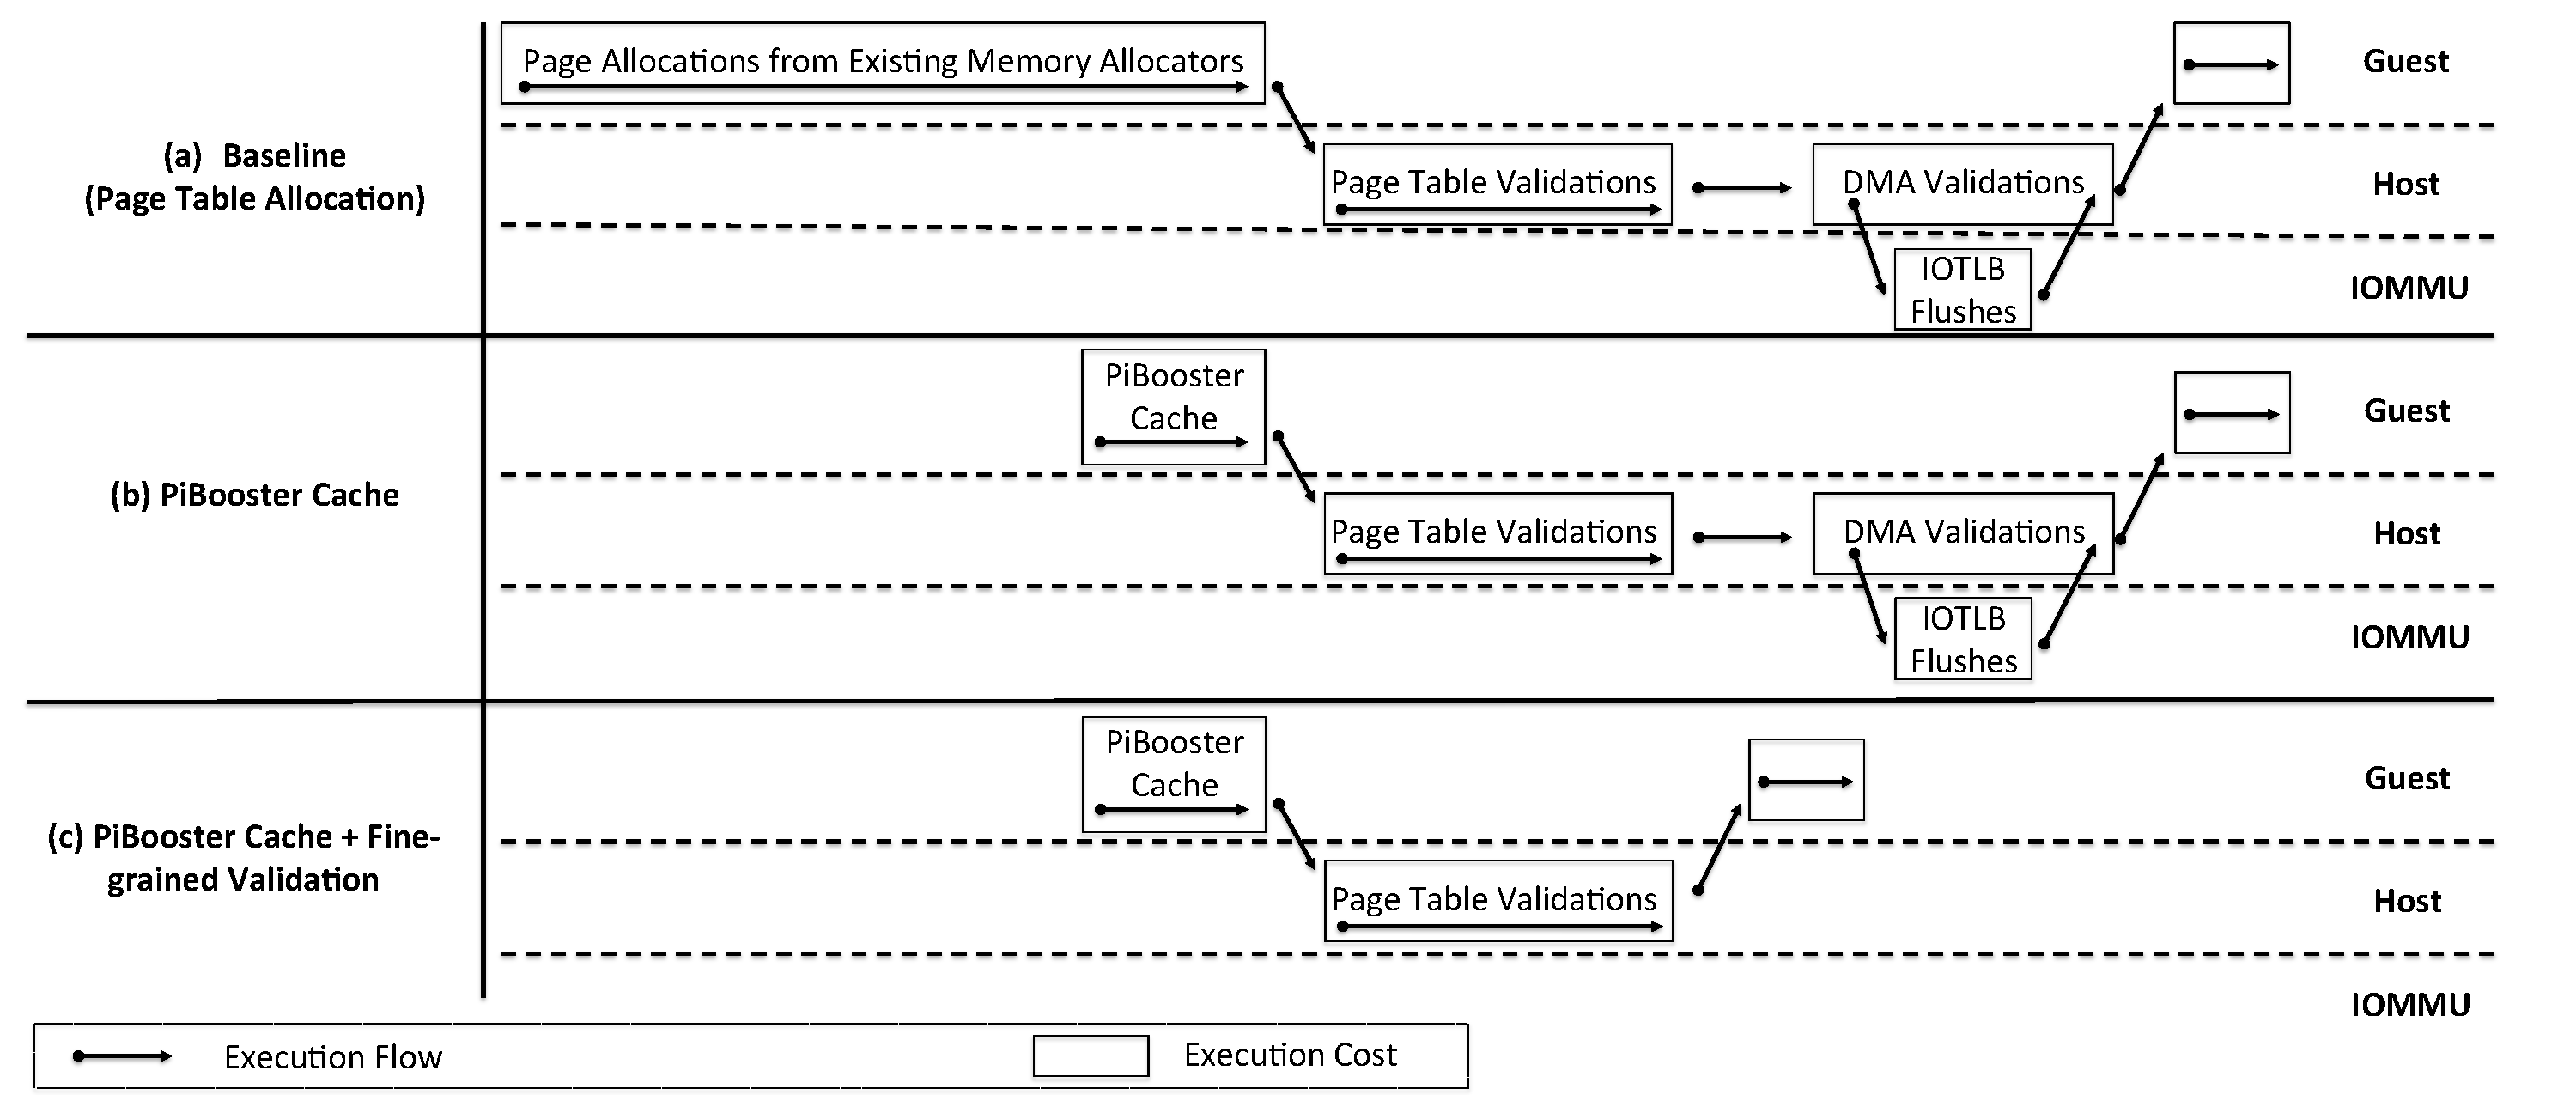
\includegraphics[width=0.9\textwidth]{image/overview/overview.pdf} \\
\caption{Solution Overview. When the \name cache and fine-gained validation mechanisms are enabled,
the execution path of page table allocation is dramatically reduced, and the additional IOTLB flushes are eliminated.}
\label{fig:overview}
\end{figure*}

%Highlight the problem, and emphasize the importance.
\mypara{Problem}
However, all existing patches mainly focus on the security enhancements of the hypervisor, without enough attentions to the performance improvements, which results in two noticeable issues.
The first one is the long execution paths of the guest page table (de)allocations, which involve the complex memory allocation process and the additional security validation procedure.
The memory allocation process frequently involves the \emph{slab} allocator~\cite{slaballocator} and the page frame allocations that are frequently managed with a buddy system~\cite{buddyallocator}, which introduces deep invocations for each page-table (de)allocation.
Moreover, the additional security validation procedure always adds extra costs for preventing malicious software and DMA accesses.
All these lead to poor performance of the page table (de)allocation, and consequently result in the long latencies of the creations and exits of processes.

The other one is the additional IOTLB flushes introduced by the security validations of the page table (de)allocations.
The guest page tables should be non-readable for any DMA requests and the corresponding pages should be readable and writable when the page tables are released.
The updates of the access permissions require IOTLB flushes to refresh the access permissions, which is necessary for the sake of the security of the hypervisor.
In addition, these access permission update events are \emph{often} triggered during the whole life cycle of a running system.
As a consequence, the IOTLB flushing events are \emph{frequently} involved, which inevitably increases the IOTLB miss rate and lowers the speed of the DMA address translation.
All these are likely to introduce negative impacts on the I/O performance of all peripheral devices.
The baseline of Figure~\ref{fig:overview}a illustrates the two issues in the page table allocation process.

\mypara{Solution}
%introduce our approach
The above identified performance issues urge us to revise the design of the page table management to improve the performance and keep the security guarantees.
In response to the appeal, in this paper we propose \name, a novel software-only approach for improving performance in page table management.
First, \name shortens the execution paths of the page table (de)allocations by \cache, which maintains a dedicated buffer for serving page table (de)allocations (Figure~\ref{fig:overview}b).
The \cache queues the deallocated page-table pages in the hope that
they will be reused (popped out of the cache) in the page table allocations in the near future.
By doing so, the page table allocations do not need to involve the costly memory management subsystem every time, instead they could directly get pages from the cached buffer.
As the functionalities of the \cache are concentrated, it is relatively easy to make it small, simple and efficient, dramatically shortening the execution path.

Second, \name eliminates the additional IOTLB flushes with a fine-grained validation scheme (Figure~\ref{fig:overview}c ), which separates the software and DMA validations.
In the traditional design, there are two types of pages: writable page that is writable for software and DMA requests, and non-writable page (e.g., page-table page) that are non-writable for both software and DMA.
The page table allocations and deallocations always involve the type changes between both of them.
Thus, the hypervisor has to do both software and DMA validations to ensure that both of them are not violating the security policies.
However, we observed that it is not necessary to do DMA validation every time if we create a new page type (i.e., semi-writable page) with non-writable permission for DMA access, and make the page type changes are only happened between the page-table pages and the semi-writable pages during the page table allocations and deallocations.
In addition, the semi-writable pages can be smoothly maintained by the \cache.

We implement a prototype on Xen with Linux as the guest kernel. We do small modifications of Xen version 4.2.1 ($166$ SLoC) and Linux kernel version 3.2.0 ($350$ SLoC).
We evaluate the I/O performance in both micro and macro ways.
The micro experiment results indicate that \name is able to completely eliminate the additional IOTLB flushes, and effectively reduce (de)allocation time of the page table.
There are (34\%, 47\%), (38\%, 22\%) and (65\%, 65\%) improvements for a pair of allocation and deallocation for three-level page table, from top to bottom.
Even in the worst cases when the \name has to go through the traditional path to allocate pages, the performance overhead for one page table allocation is still very small, only adding about 20 instructions. Fortunately, the worst cases are rarely happened. According to our experiment results, the number of worst cases is only $348$, out of the total allocation requests (i.e., $198990$), in 30 minutes execution.
The macro benchmarks show that \name has no negative impact on the CPU computation, network I/O and disk I/O.
In particular, the latencies of the process creations and exits are expectedly reduced by 16\% on average.

In summary, we make the following contributions:
\begin{enumerate}
\item We identify two significant performance issues in the page table management. In particular, we are the first, to the best of our knowledge, to identify the performance issue between guest page table (de)allocations and the IOTLB flushes.
\item We proposed a novel approach - called \name, to shorten the execution paths of the page table allocation and deallocations, and eliminate the additional IOTLB flushes, without sacrificing the system security.
\item We implemented a prototype of the page table cache and evaluated the performance in both micro and macro ways. The experiment results indicate that the \name can benefit the page table (de)allocations, without negative performance impacts on the system.
\end{enumerate}

The rest of the paper is structured as follows: In Section~\ref{sec:prob}, we briefly describe the background knowledge, and highlight the performance issues. Then we describe the system overview and implementation in Section~\ref{sec:overview} and Section~\ref{sec:impl}. In Section~\ref{sec:eva}, we evaluate the performance of the \name system, and discuss several issues in Section~\ref{sec:dis}. At last, we discuss the related work in Section~\ref{sec:related}, and conclude the whole paper in Section~\ref{sec:con}.


\section{Problem Definition} \label{sec:prob}
In this section, we describe the necessary background knowledge and highlight the identified two performance issues: 1) long execution paths of the guest page table (de)allocation and 2) the additional IOTLB flushes.
As Xen~\cite{XEN-SOSP03} is a typical and popular paravirtual hypervisor, we use Xen in a x86 MMU model~\cite{x86-pv-model} to illustrate the details.
The presented or similar mechanisms are available on the other paravirtual settings.


\subsection{Long Execution Path}\label{sec:longpath}
The long execution path issue refers to the execution paths for the guest page table page allocation and deallocation.
In the existing design, allocating and deallocating a page table page are time costly, as they have to invoke the complex memory allocators and performance both software (i.e., page table) and DMA validations.
%In addition, the DMA validations always lead to additional IOTLB flushes, which would reduce the DMA address translation speed and may consequently lower the I/O performances.
In addition, such allocation and deallocation events frequently occur in the system, i.e., the numerous process creations and exits will result in many page-table page allocations and deallocations.
Thus, it is necessary to deeply understand the long execution path issue and improve the performance accordingly.

\subsubsection{Page Allocation and Deallocation}
To allocate a page, the guest kernel has to invoke the system allocators, typically from slab allocator to buddy allocator.
The slab allocator~\cite{slaballocator} consists of a variable number of caches that are linked together on a doubly linked circular list.
Each cache maintains blocks of contiguous pages in memory called slabs, which are carved up into small chunks for the data structures and objects.
When \emph{kmalloc} is called, all it does is searching through the prepared caches.
If there is no suitable object, the buddy allocator will be involved.
The Buddy allocator~\cite{buddyallocator} manages all free pages that are managed in blocks as a power of 2.
When the allocation function is invoked, it first searches for the block of the requested size.
If no expected block is free, the allocator will continue to search for the block of the next size (which is twice that of the requested size).
This process continues until all of the free area has been searched or until a block has been found.

In contrast to the page allocation, the page deallocation is to return the page back to the system.
The deallocation process may also invoke slab allocator and/or buddy allocator, and would trigger the updates of the corresponding data structures,
e.g., the buddy allocator always attempts to recombine the freed pages into larger blocks.

In brief, the page allocation and deallocation are time costly due to the deep invocations and complex updates of the dependent data structures.


\subsubsection{Page Table Validations}\label{sec:pv-security}
Page tables are used by a hardware, i.e., Memory Management Unit (MMU), to translate the linear addresses into physical addresses used by the hardware to execute instructions.
In the PAE-enabled paging mode, a page table has three levels: L1 level (bottom level), L2 level (middle level) and L3 level (top level).
The slots in L1, L2 and L3 levels are known as Page Table Entry (PTE), Page Middle Directory (PMD) and Page Global Directory (PGD), respectively.
A PTE slot could determine the access permissions of a page, e.g., the kernel could set a page as read-only by clearing the bit within a PTE slot that represents the writable permission.
Typically, each user process has its own page table, and the creation and exit of a user process will be accompanied by the allocation and deallocation of a page table respectively.
\begin{figure}[ht]
\centering
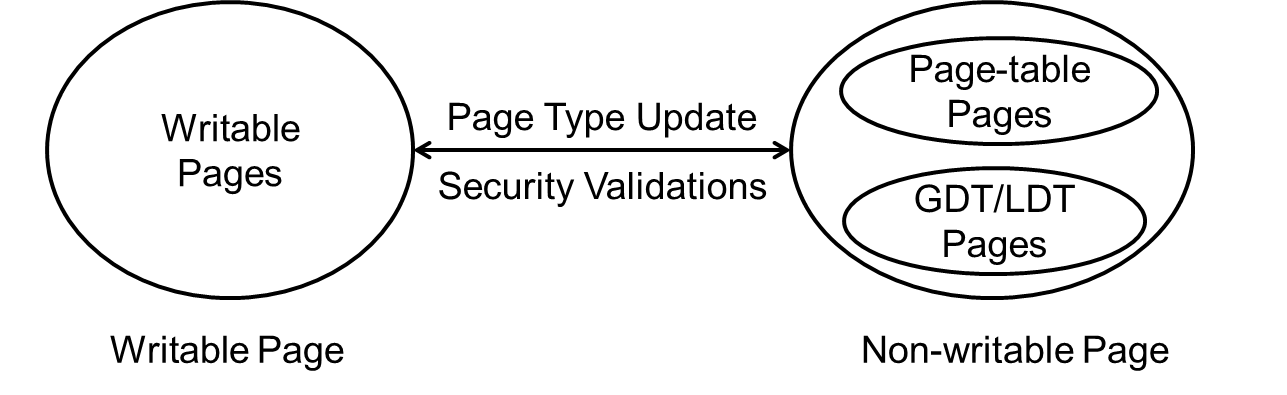
\includegraphics[width=0.45\textwidth]{image/background/page-type-update.png} \\
\caption{Page type updates between writable pages and non-writable pages. }
\label{fig:page-type-updates}
\end{figure}


%In order to ensure that the guest cannot subvert the system, the hypervisor requires that certain update policies are maintained,
%and thus all updates of the page tables should be vetted by the hypervisor.
%To this end, the guest OS is deprivileged, from ring-0 to ring-1, leaving ring-0 for the Xen hypervisor.
%This prevents the guest OS from executing privileged instructions, e.g., the guest OS cannot directly update control registers.

The hypervisor defines two page types 1) \emph{writable page} that is writable for software and DMA, and 2) \emph{non-writable page} that is non-writable for both software and DMA.
The non-writable page has several sub-page types, such as page-table page and GDT/LDT pages.
In addition, the hypervisor also requires that every page type update only occur between writable and non-writable pages, as summarized in Figure~\ref{fig:page-type-updates}.
The hypervisor maintains a type reference count for each page, and enforces the policy that any given page has exactly one type at any given time.
In addition, it also enforces that only pages with the writable type have a writable mapping in the page tables.
By doing this it can ensure that the guest OS is not able to directly modify any page-table pages and therefore cannot subvert the security of the whole system.

Whenever a page table is loaded to work, there should be a page type update from writable page to non-writable page (i.e., page-table page).
First, the hypervisor must ensure the L3 page-table page has a type count of zero.
In addition, it must be validated to ensure that it follows the following policy:
for a page with a page-table type to be valid, it is required that any pages referenced
by a present page table entry in the page have the type of the next level down.
For instance, any page referenced by a page with type L3 Page Table must itself have the type L2 Page Table.
This policy is applied recursively down to the L1 page table layer.
At L1 the invariant is that any data page mapped by a writable page table entry must have the writable page type.
By applying these policies, Xen ensures that all page-table pages as a whole are safe to be loaded.
The hypervisor also verifies all slots of the page table to ensure that the mappings and access permissions are correct and expected.
Note that the hypervisor is always involved in all updates of the page tables, the policies on the page table updates are non-bypassable.

The validation process in the page table deallocation is contrary to the one in the page table allocation.
In brief, the hypervisor will validate the page table's type count, access permissions and the slot mappings to ensure that the page table is completely and securely deallocated.

\subsection{DMA Validations and IOTLB Flushes}
\subsubsection{DMA Address Translation}
The input/output memory management unit (IOMMU)~\cite{intelvt} is a memory management unit (MMU) that connects a DMA-capable I/O bus to the main memory.
Like a traditional MMU, the IOMMU maps device addresses (also called as I/O addresses) to physical addresses through a dedicated page table.
%This technique is also known as DMA remapping.
The IOMMU page table that is created and maintained by the hypervisor in its own space is able to restrict the access on a particular page by configuring the permission bits.
The hypervisor grants different access permissions for different page types, such as the writable pages are always allowed with full access permissions, while the page-table pages are always inaccessible to any devices.

However, if the DMA address translation always needs to look up the IOMMU page table, it will be slow and inefficient.
To accelerate the translation speed, the I/O translation look-aside buffer (IOTLB) is introduced.
The IOTLB is used to cache frequently accessed page table entries.
By doing so, the IOTLB is very likely to be accessed, indicating that the physical address of a queried DMA address will be immediately fetched through the IOTLB path (Figure~\ref{fig:iotlbpath}).
If unlikely the IOTLB miss occurs, the DMA address translation still can go the slow I/O page-table path to get the physical address (Figure~\ref{fig:ioptpath}).
To achieve a better I/O performance, the DMA address translation should avoid taking the I/O page-table path as far as possible.

\begin{figure}[!t]
    \begin{subfigure}{0.45\textwidth}
        
\includegraphics[width=1\textwidth]{image/background/DMA-IOTLB-translation.png}
        \caption{\centering IOTLB Path.}
        \label{fig:iotlbpath}
    \end{subfigure}
    \vfill
    \begin{subfigure}{0.45\textwidth}
        
\includegraphics[width=1\textwidth]{image/background/DMA-pt-translation.png}
        \caption{\centering I/O Page-Table Path.}
        \label{fig:ioptpath}
    \end{subfigure}
    \caption{IOTLB path is much faster than I/O page-table path.}
    \label{fig:dma-add-trans}
\end{figure}


\subsubsection{Additional IOTLB Flushes}
%In paravirtualization, the writable page is writable for DMA requests, while the non-writable page (e.g., the page table page) is non-writable for DMA requests.
The page table allocation and deallocation always trigger the updates between the writable pages and the page-table pages, and they have different access permission for DMA requests.
To keep the security of the hypervisor, the DMA validation is necessary.
Specifically, the hypervisor will update the corresponding entries of the IOMMU page table to set correct access permissions.
After this, the hypervisor also needs to flush IOTLB entries to invalidate the old entries, without which the security of the hypervisor would be violated, e.g., the DMA requests could write the page-table pages through stale IOTLB entries.

\begin{figure}[ht]
\centering
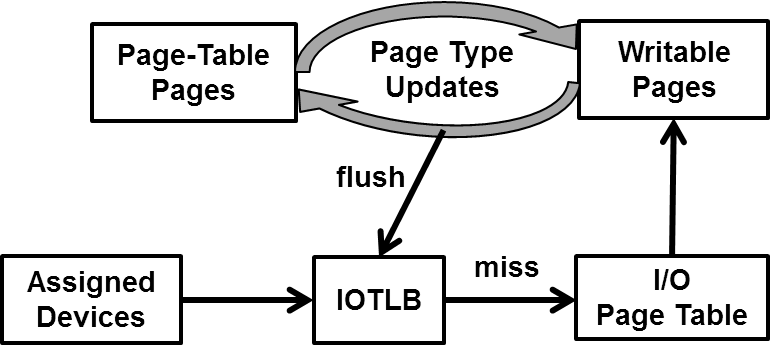
\includegraphics[width=0.45\textwidth]{image/background/problem-illustration.png} \\
\caption{The DMA validations in page type updates introduce additional IOTLB flushes, which lead to selecting the slow path  (i.e., I/O page-table path) of the DMA address translation.}
\label{fig:pro-ill}
\end{figure}


In addition, the additional IOTLB flushes are likely to let the DMA address
translations take the slow and inefficient page-table path,
instead of taking the fast and efficient IOTLB path (Figure~\ref{fig:pro-ill}), due to the additional IOTLB misses.
Numerous IOTLB misses would lower the speed of the DMA transferring, especially for the high performance devices, such as the Intel I/OAT ~\cite{lauritzenintel}.
%Moreover, the DMA validations are frequently triggered if there are many creations and exits of user processes due to certain cases.
%In fact, it


%In brief, we summarize all these into three key points, which are listed as follows:
%\begin{enumerate}
%\item (O1) Each page-type change triggers the invalidation of at least one IOTLB entry.
%\item (O2) The main source of causing IOTLB flush is the page-type changes between writable pages and page-table pages (see figure~\ref{fig:pro-ill}).
%\item (O3) The additional IOTLB flushes inevitably have negative impacts on the I/O performance of the peripheral devices.
%\end{enumerate}



\section{\name Overview} \label{sec:overview}
\begin{figure*}[ht]
\centering
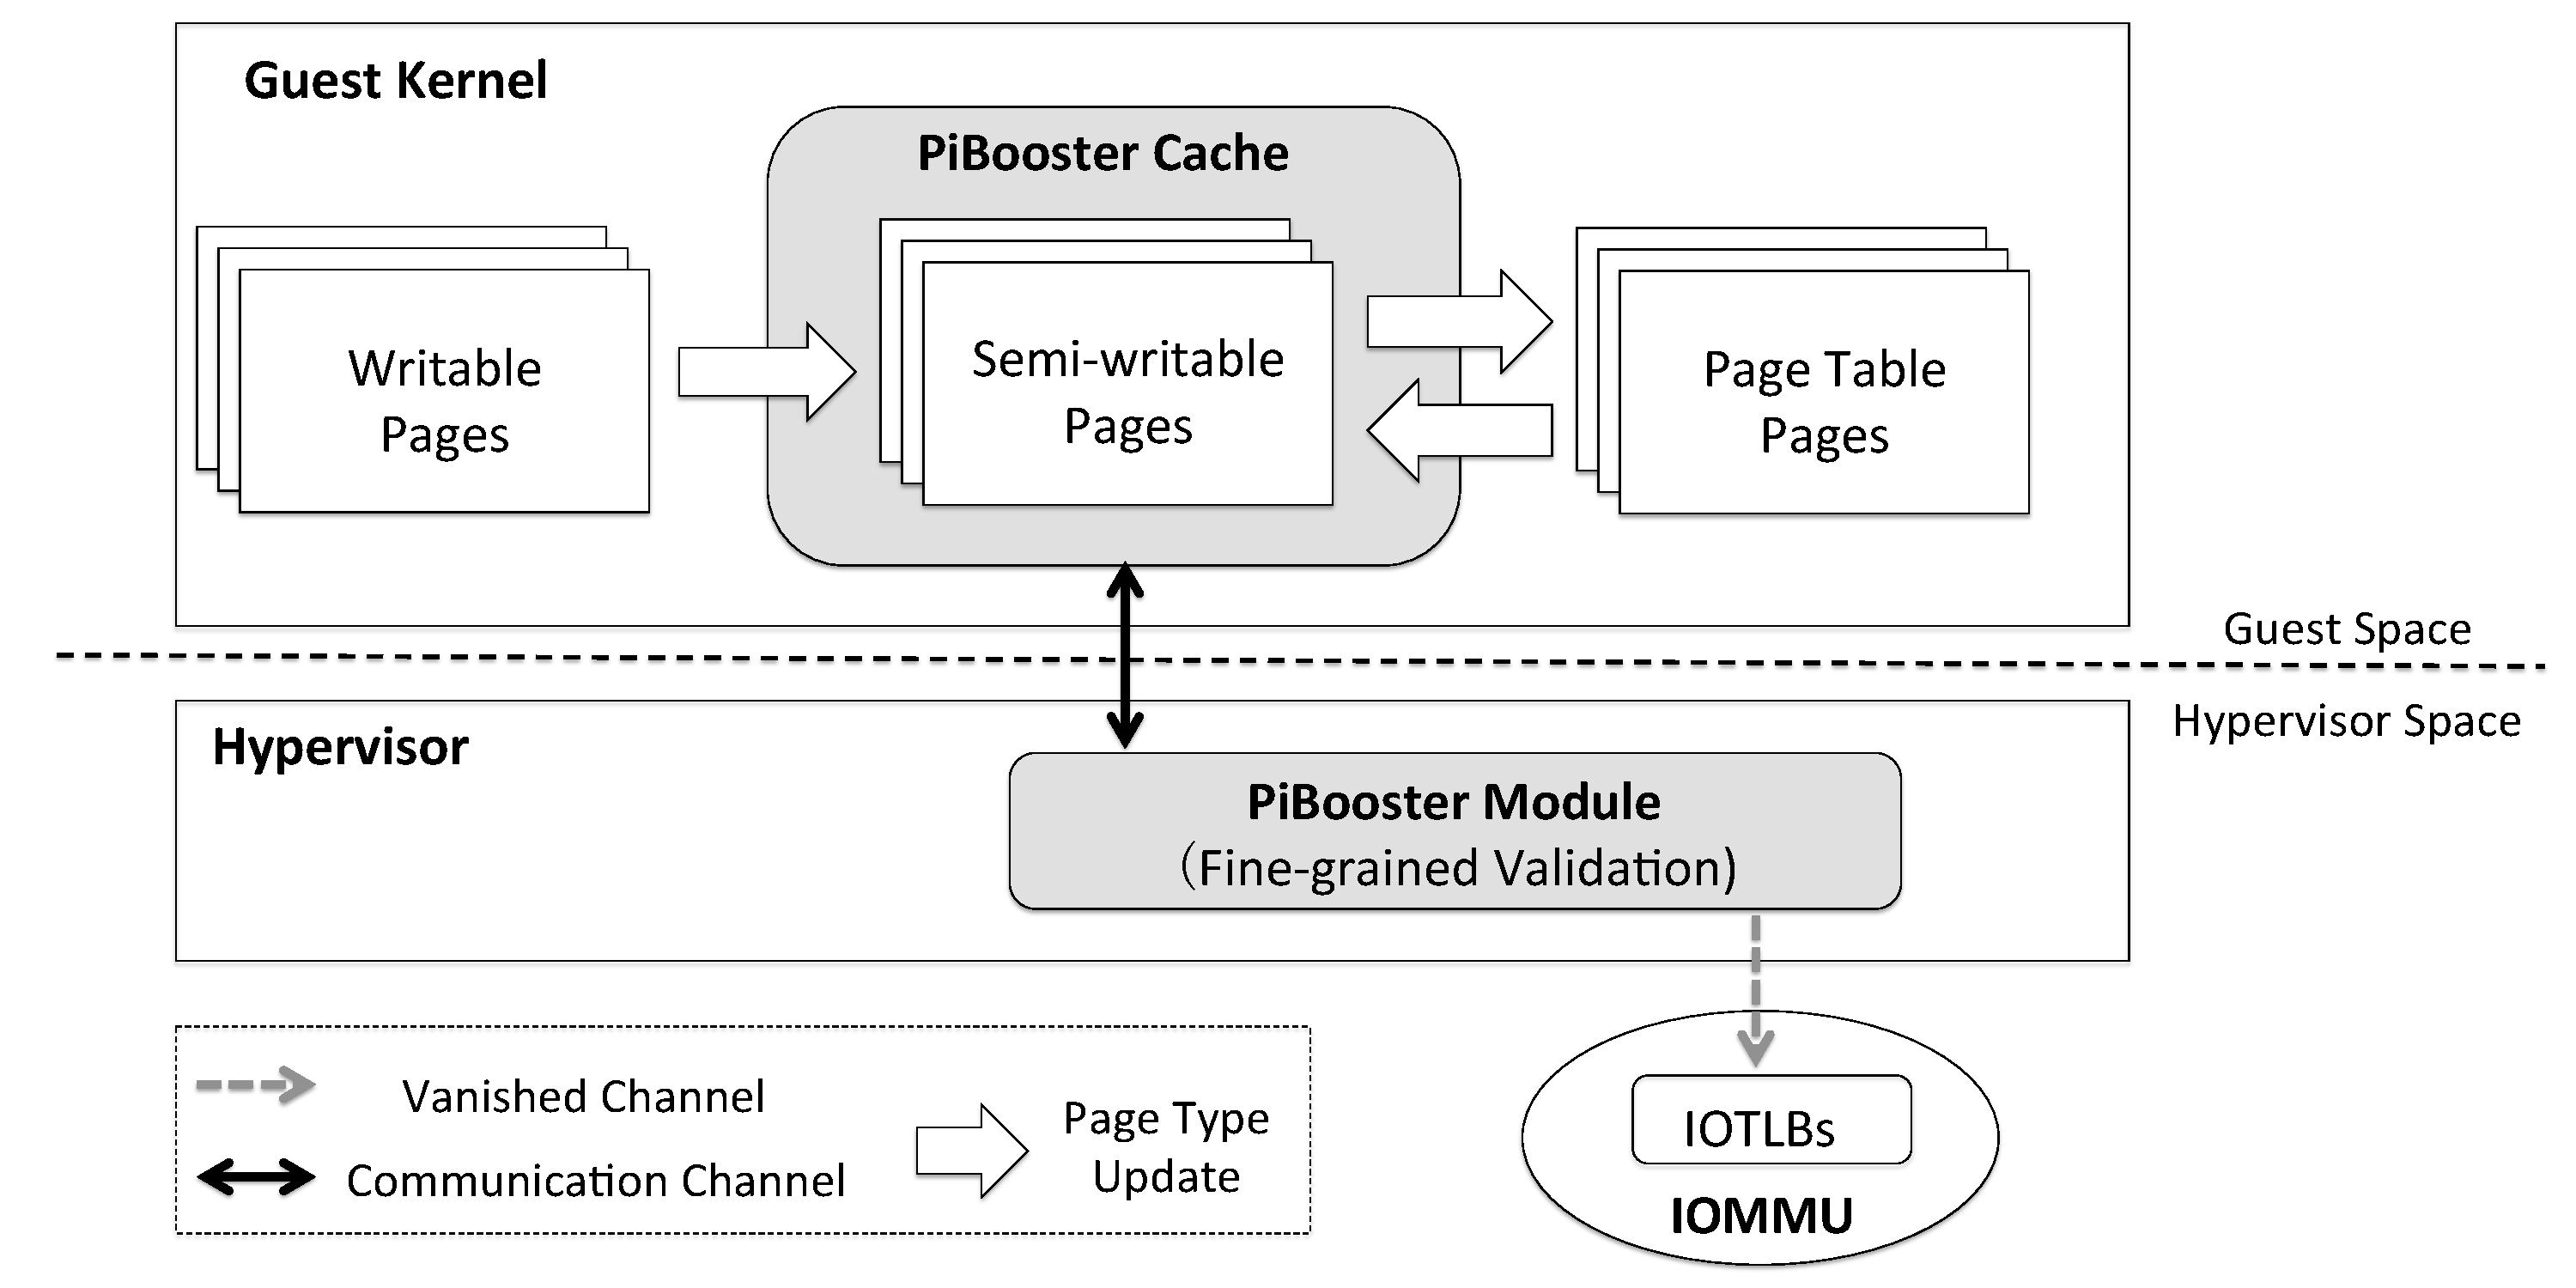
\includegraphics[width=0.8\textwidth]{image/overview/arch.pdf} \\
\caption{\name Architecture. The semi-writable pages are managed by the \name cache, and all page type updates are validated by the \name module.
Through the cooperation of \name cache and \name module, \name successfully shortens the execution paths of the guest page table (de)allocations and eliminates additional IOTLB flushes.}
\label{fig:arch}
\end{figure*}

\subsection{Design Requirements}\label{sec:req}
In the design of \name, we consider several requirements, which are summarized and listed as follows.
\begin{enumerate}
\item Unaltered system security. The new scheme should not sacrifice the system security to obtain benefits from I/O performance. No one likes to use a system with known design loopholes.
\item Compatible with legacy applications. The new scheme should limit the modifications on the guest kernel and the hypervisor, without any modifications on the existing applications.
\item Small modifications. The new scheme should minimize the development cost on the guest kernel and the hypervisor.
\item Minimizing additional IOTLB flushes. The new scheme should minimize the number of IOTLB flushes, such as reducing the number to zero.
\end{enumerate}

\subsection{\name Architecture}
Figure~\ref{fig:arch} depicts the architecture of \name. It consists of a \cache in the guest kernel and a \name module in the hypervisor space.
%the mechanism of the \cache
The \cache allocates a number of semi-writable pages at the initial stage,  which are newly introduced by the fine-grained validation scheme (Section~\ref{sec:fine-grained}).
These semi-writable pages are maintained in a dedicated cache.
At runtime, the \cache attempts to satisfy all page table allocation and deallocation requests, shortening the execution path and saving the execution time.
There are many page type updates from/to the semi-writable pages.
The \cache mediates these updates and issues hypercalls to the hypervisor, asking it to perform the fine-gained security validations on the update requests (i.e., the communication channel).
Once the verified pages pass the validations, their page types will be updated accordingly.
%The guest kernel cannot bypass the security validation process, as the hypervisor is the only one to determine/update the page type.

The \module enforces the fine-grained validation scheme on the page table updates.
It performs (1) the page table validations that validate the page table contents as well as the type count, and (2) the DMA validations that ensure that the DMA requests cannot write the page-table pages and the semi-writable pages.
In the traditional validation scheme, the DMA validations always triggers the additional IOTLB flushes due to the access permission updates between the writable pages and the page-table pages.
In the fine-grained validation scheme, both semi-writable pages and page-table pages are non-writable for DMA requests.
Thus, the hypervisor never needs to do the IOTLB flushes or IOMMU page table updates (i.e., vanished channel), which will benefit the I/O performance of the peripheral devices.
Moreover, it also saves the time of the whole security validation, further reducing the execution time of the page table allocations and deallocations.

\subsection{Fine-Grained Validation}\label{sec:fine-grained}
%To reduce the number of the IOTLB flushes, a possible approach is to let the hypervisor to manage the page table in its own space.
%In this way, there is no need for flushing IOTLB, but it will dramatically increase the size of the hypervisor, and consequently reduce the system security level.
%Another possible approach is to do the IOTLB flushing in a batch, meaning flushing multiple IOTLB entries all in one, instead of flushing them one after another.
%This approach is able to retain the system security, but it could not eliminate the IOTLB flushes, only reducing the number of IOTLB flushes in a certain level.
%In addition, this approach may result in security loopholes as the IOTLB entries are not synchronized with the corresponding IOMMU page table slots.
The fine-grained validation scheme aims to eliminate the additional IOTLB flushes and reduces the total time of the security validations.
Specifically, in the traditional security validation scheme, there are only two general page types: writable page and non-writable page,
and the type updates between them are required to do both page table validations and DMA validations.
The DMA validations not only increase the total validation time, but also introduce numerous additional IOTLB flushes.
%, which are likely to reduce the I/O performance of all related peripheral devices.
Moreover, the additional IOTLB flushes cannot be skipped, because it would provide a time gap for the adversary to attack the hypervisor by leveraging the stale IOTLB entries.
%1) bad impacts of original coarse-grained validation scheme 1) additional IOTLB flushes, and 2) long validation process

%2) How to do the fine-grained validation 1) semi-writable page 2) new page type updates 3) why save time and eliminate IOTLB flushes
To address this problem without sacrificing the system security, we introduce a new page type: \emph{semi-writable page}, which is writable for software but non-writable for DMA.
In addition, we enforce that the page type updates between the writable page and the page-table page must go through the semi-writable page first (as illustrated in Figure~\ref{fig:arch}).
As the semi-writable page and page-table page are already inaccessible to DMA, there is no need to do the DMA validations, meaning that the additional IOTLB flushes could be totally avoided.
As a consequence, the time of the whole security validation process is reduced, accelerating the speeds of page table allocations and deallocations.
%In order to facilitate the management of the semi-writable pages, we propose a cache, called \cache, in the guest kernel, and extend the existing page management data structure in the hypervisor space.
Similar to the management of the page-table pages, the hypervisor is only responsible for the final validation of the semi-writable page, leaving all other management operations for the \cache.
By doing this, we can keep the modifications as small as possible by reusing existing validation process and page-table management subsystem, and also retain the system security.


\subsection{\name Module}\label{sec:module}
The \module works in the hypervisor space, extended from the original coarse-gained validation module.
The first task of the \module is to trace the page type.
Instead of adding a new data structure for tracing the semi-writable pages, the \module chooses to reuse the existing ones.
By extending the existing page-type data structure, the \module adds a new bit for \emph{semi-writable page}.
By doing so, the \module could reuse all existing interfaces.

The second task of the \module is perform the security validations on all page type update requests.
The purpose of the security validations is to prevent software and DMA attacks on the hypervisor.
As the semi-writable pages are writable for the guest OS, the updates on the page table may violate the security policies. Thus, the page table validations are always necessary.
However, the DMA validations can be skipped, as both semi-writable page and page-table page are non-writable for DMA.
This is why the page type updates between two of them do not trigger any additional IOTLB flushes.

The \module also exports a new hypercall interface for the \cache to facilitate their communications.
Through the new interface, the \cache could explicitly invoke the \module to perform the security validation according to its demand.

\subsection{\name Cache}\label{sec:cache}
The basic idea behind the \cache is to have caches of semi-writable pages available for page table allocations and deallocations.
Without the page oriented \cache, the kernel will spend much of its time allocating, initializing and freeing page-table pages.
The slab allocator that is similar to the \cache is not used in our settings, due to the following reasons.
%unaware of the page type updates
First, it violates one of security requirements of the page-table pages enforced by the hypervisor.
In particular, the type count should be zero when a page is updated among the writable page, the semi-writable page and the page-table page.
However, the pages in the slab allocator do not always satisfy this restriction, as it may build multiple mappings for one page.

Second, the existing size-oriented management of the slab does not distinguish the page-table pages from other pages that have the same size, and the customization of this management mechanism would need lots of development costs, such as interface updates, internal data structure updates.
In addition, the related components that rely on the slab allocators may also be affected.
At last, adding the fine-grained validation mechanism only for one object (i.e., page-table page) will subvert the generality of the slab allocator.
Considering the above three reasons, we give up reusing the existing slab allocator and aim to build a dedicated one, called \cache, for page table allocation and deallocation.

\subsubsection{\name Cache Initialization and Destruction}
The \cache is enabled in the system bootup phase by default.
By doing so, the page tables of all user processes are maintained by the \cache from the very beginning.
To increase the flexibility, it is also allowed to dynamically enable it at runtime through the prepared interface.

In the initialization phase, the \cache allocates several pages from writable pages using existing system allocators, converts them into semi-writable pages, and maintains them in a dedicated cache list.
At runtime, the page table deallocations are always successful by efficiently pushing deallocated pages into the \cache.
When the guest kernel needs page-table pages, the \cache will pop out the cached pages to satisfy the requirements.
In certain worst cases (e.g., many allocation requests but only a few or no deallocations), if the cached pages cannot satisfy the requests of page table allocations, the \cache has to re-invoke the system allocators to get new ones. 
Fortunately, the re-invocations rarely happen in a workflow-stable system.
In fact, there are always multiple semi-writable pages in the \cache that are ready for page-table allocations after the system is running for a few minutes in our experiments. Such cases will be evaluated in Section~\ref{sec:eva}.

The \cache works in the whole life cycle of the guest by default, but the end  user is able to explicitly disable it at any time through the exported interface.
Once the \cache receives the \emph{disable} command, it will release all resources, e.g., deallocating the cached pages assisted by the existing system allocators as well as the \module, and releasing the data structures that are used for managing the cached pages.
In addition, it will also issue a hypercall to inform the hypervisor, which will disable the fine-grained validation mechanism and switch back to the original coarse-grained validation scheme.
%As the disable costs are quite high, we recommend that always keeping the \name running once it starts to work.

\subsubsection{Cache Shrinking}
When the memory management daemon (e.g., \emph{kswapd}) notices that memory is tight, it will explicitly call the exported interfaces of the \cache to free some memory.
%talk about the interface
There are two interfaces to shrink the cache pages. One is based on the page number. The memory management daemon can specify a number to ask the \cache to release.
The other one is based on the percentage. For instance, the kernel could ask the \cache to release 50\% cached pages.
%the size of the cache.
In fact, the number of semi-writable pages maintained in the \cache is not too high. In our experiments, it is always less than $180$, meaning that the size of the cache is less than $720KB$.

The \cache could also automatically shrink itself through the predefined threshold.
The threshold can be defined according to the page number or the proportion (i.e., the number of the cached semi-writable pages over the number of the page-table pages), or the combination of them.
%In the current prototype, the threshold is the combination of the page number and the percentage.







\section{Implementation} \label{sec:impl}
\yueqiang {
implementations:
1) hooks for on-demand enable
2) locks for mechanism
3) data structures in mechanism
4) threshold selection for cache free? or this discussed in design
5) }

Based on guest kernel version 3.2.0 and Xen version 4.2.1, \name implements the cache and the fine-grained validation module.

\subsection{\name Find-grained Validation Module}

\begin{figure}[ht]
\centering
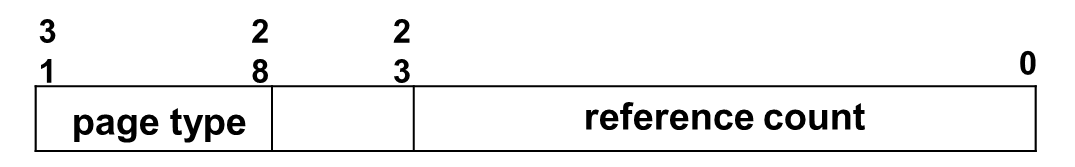
\includegraphics[width=0.45\textwidth]{image/implementation/field-of-page-type-info.png} \\
\caption{Field of Page Type Info}
\label{fig:field-of-page-type-info}
\end{figure}

From a 32-bit field related to page type information, \name was planning to use a redundant bit to represent the cache flag in order to be compatible with its original implementation. However, each bit in the upper 9-bit of the field has its specific use and the lower 23-bit serves as the reference count of current page type, representing at most ($2^{23}-1$) reference counts of the page type (see figure~\ref{fig:field-of-page-type-info}). \name enforces a stricter rule to prevent count overflow, as cache flag occupies the top bit of the 23-bit and the maximal reference count is limited to ($2^{22}-1$), which affects Xen little (see figure ~\ref{fig:field-of-semi-type}). Actually, Xen hypervisor is functioning well with the flag bit since the reference count of a page type during runtime cannot reach at ($2^{22}-1$). On top of that, \_\_get\_page\_type() is the critical function to be customized in order to check if a machine page has the flag bit.

\begin{figure}[ht]
\centering
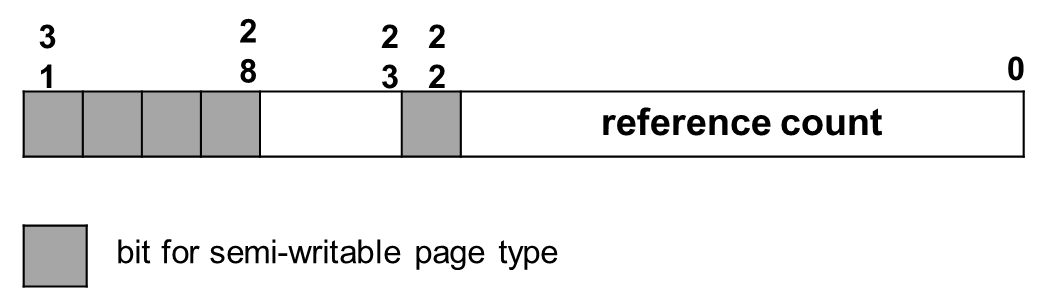
\includegraphics[width=0.45\textwidth]{image/implementation/field-of-semi-type.png} \\
\caption{Representation of Semi-Writable Page Type}
\label{fig:field-of-semi-type}
\end{figure}

\subsection{\name Cache}

In the PV setting, guest OS is required to work in PAE (i.e., Physical Address Extension) mode. As a result, \name maintains three levels of cache pools, each of which is essentially a structured single-linked list caching the guest physical addresses of pages. For the top two levels used for caching PGD (i.e., Page Global Directory) and PMD (i.e., Page Middle Directory), \name obtains the physical addresses directly from their linear addresses. While the bottom PT (i.e., Page Table) is located in the High Memory, the mapping between its linear and physical addresses is not stable. \name acquires the physical addresses of cached PT pages from the corresponding page-info structures.

Every list supports operations of both removal and insertion. Removal exists within the cache allocating function, which fetches a cached page from the top of the list. Insertion is located within the cache freeing function, which inserts a cached page also onto the top. Also, \name maintains two global operation counters, namely num\_in\_use and num\_in\_pool, each logging the invocation times of removal and insertion, respectively. They are required when cache freeing function needs to free cached pages into the buddy system. Every pair of cache allocating and freeing functions is used to hook existing page-table related functions. By this way, whenever OS creates or destroys any process, it always interacts with the caches. Also note that every cache pool and operation counter are shared data resources and their related operation code are critical sections. \name makes use of locks to ensure exclusive resource-access in the multi-processor setting. More specifically, Every level of page-table cache and all its operation counters share a spin lock and irrelevant operations should be removed out of the critical section, especially those that are time-consuming.

\name implements a new system call to provide an interface for users to activate the cache in an on-demand way. In the system call, a global boolean variant is defined, which is initialized as false, indicating that cache is not enabled. And users can assign the variant as true to enable the cache. Anther two user interfaces related to modification of default thresholds and freeing all pages in cache are also implemented through system calls. For the modification, new thresholds of the proportion and total page number are passed as agruments while users can frees all cached pages by resetting a global boolean variant, which is initialized as true.

Within the cache freeing function, a hypercall is implemented with a single-linked list of cached addresses of pages as the parameter. The hypercall is a uniform interface for every level of cache freeing function, simplifying the modifications both to guest OS and Xen. As a reply to the hypercall, Xen mainly zeroes the flag bit of 32-bit field and invokes the important function interface intel\_iommu\_map\_page to create entries in the I/O page tables as well as flush IOTLBs.


% TEMPLATE for Usenix papers, specifically to meet requirements of
%  USENIX '05
% originally a template for producing IEEE-format articles using LaTeX.
%   written by Matthew Ward, CS Department, Worcester Polytechnic Institute.
% adapted by David Beazley for his excellent SWIG paper in Proceedings,
%   Tcl 96
% turned into a smartass generic template by De Clarke, with thanks to
%   both the above pioneers
% use at your own risk.  Complaints to /dev/null.
% make it two column with no page numbering, default is 10 point

% Munged by Fred Douglis <douglis@research.att.com> 10/97 to separate
% the .sty file from the LaTeX source template, so that people can
% more easily include the .sty file into an existing document.  Also
% changed to more closely follow the style guidelines as represented
\section{Evaluation} \label{sec:eva}
%
We have implemented the proposed prototype demonstrated in previous sections. The implementation added or changed %$350$ SLoC to Linux kernel and $166$ SLoc to Xen hypervisor, of which $2$ SLoc in the hypervisor are
$166$ SLoc of Xen hypervisor and $350$ SLoC of Linux kernel.
This section evaluates the performance of \name by running both micro- and macro-benchmark kits.

\subsection{Experimental Setup}

Our experimental platform is a LENOVO QiTianM4390 PC with Intel Core i5-3470 running at 3.20 GHz, four CPU cores available to the system. We enable the Intel VT-d feature in the BIOS menu, which supports queue-based invalidation interface in the granularity of page invalidation. Xen version 4.2.1 is used as the hypervisor while \emph{domain 0} uses the Ubuntu version 12.04 and kernel version 3.2.0. Besides, \emph{domain 0} configures its grub.conf to enable DMA address translation mode of IOMMU and to print log information to a serial port in debug mode.

In the original design of Xen, page table (de)allocations will give rise to page type updates, upon which the function iotlb\_flush\_qi will be invoked to flush corresponding IOTLB entries. Thus, a global counter is placed into the function body to record invocation times of the function and then an average counter per minute is calculated as a frequency of IOTLB-flush. When the IOTLB-flush stays at zero level, it means that no page table is (de)allocated, indicating that no process creation/exit occurs then. In a nutshell, there exists a mutually positive effect between a process creation/exit and IOTLB-flush.

Because of that, we define two different system states, classified by the frequency of IOTLB-flush.

\emph{idle state}: When the system boots up and logins into the graphical desktop, lots of system processes are created, causing many IOTLB flushes. But as time goes by, the frequency of IOTLB-flush reduces rapidly and stays stable to zero level ten minutes later, and we think that system starts to be in an \emph{idle state}, where no new process creation/exit does occur while existing system daemons are still running.

\emph{busy state}: A stress tool emulating a concurrent-processes workload is developed to make the system become \emph{busy}. Specifically, the tool is busy periodically launching a default browser(e.g., Mozilla Firefox 31.0 in the experiment), opening new tabs one by one and then closing the browser gracefully in an infinite loop, so as to constantly create/terminate a large number of Firefox processes, thus giving rise to frequent page type updates of page tables. More specifically, one iteration of the loop costs five minutes and the frequencies of process creation and exit are $542.14$ times per minute and $542.07$ times per minute, respectively. Besides, the memory usage of the tool on an average iteration is $284.1$ MB. Please note that since the frequency of IOTLB-flush will become stable five minutes after the tool is launched, time period of one iteration is also set to that interval to achieve a stable frequency of IOTLB-flush.

Both micro- and macro-benchmark kits are performed under the \emph{busy state}, in which micro tests are utilized to evaluate the frequency of IOTLB-flush, CPU usage and memory size while macro-benchmarks give an assessment on overall system performance.

\subsection{Micro-Benchmarks}

Micro-experiments are conducted in three groups. In a baseline group, the \emph{idle} system enters into the \emph{busy state} under Xen's original design. On the contrary, in a pre-\name group, \name is enabled before system becomes \emph{busy}. Besides, in another group of dyn-\name, \name is dynamically enabled (e.g., five minutes after the tool is invoked) so as to evaluate the performance of dyn-\name compared to the other groups.

\begin{figure}[ht]
\centering
%\includegraphics[scale=0.55]{image/iotlbflush.png} \\
\includegraphics[width=0.5\textwidth]{image/micro/iotlbflush.png} \\
\caption{Frequency of IOTLB-flush in the pre-\name group is reduced to zero within one minute. If \name is dynamically enabled when IOTLB is flushing frequently, the frequency drops sharply within two minutes from the high level to zero and remains unchanged since then, contrary to that of the baseline group.}
\label{fig:iotlbflush}
\end{figure}

As can be seen from Figure~\ref{fig:iotlbflush}. Y-axis represents the frequency of IOTLB-flush, corresponding to the time period (i.e., one minute) of x-axis for the first thirty minutes that the \emph{busy state} lasts. From this figure, frequency in the baseline group increases rapidly and remains stable five minutes later. By contrast, frequency in the pre-\name group drops to zero level in a very short time. It can be safely concluded that the fine-grained validation module proposed by \name does eliminate the IOTLB flushes caused by concurrent processes creations/exits. The dyn-\name group shows that the frequency also can be dropped to zero level very quickly even if the system is already in a \emph{busy state}.

\begin{figure*}[t!]
    \centering
    \begin{subfigure}[t]{0.5\textwidth}
        \centering
        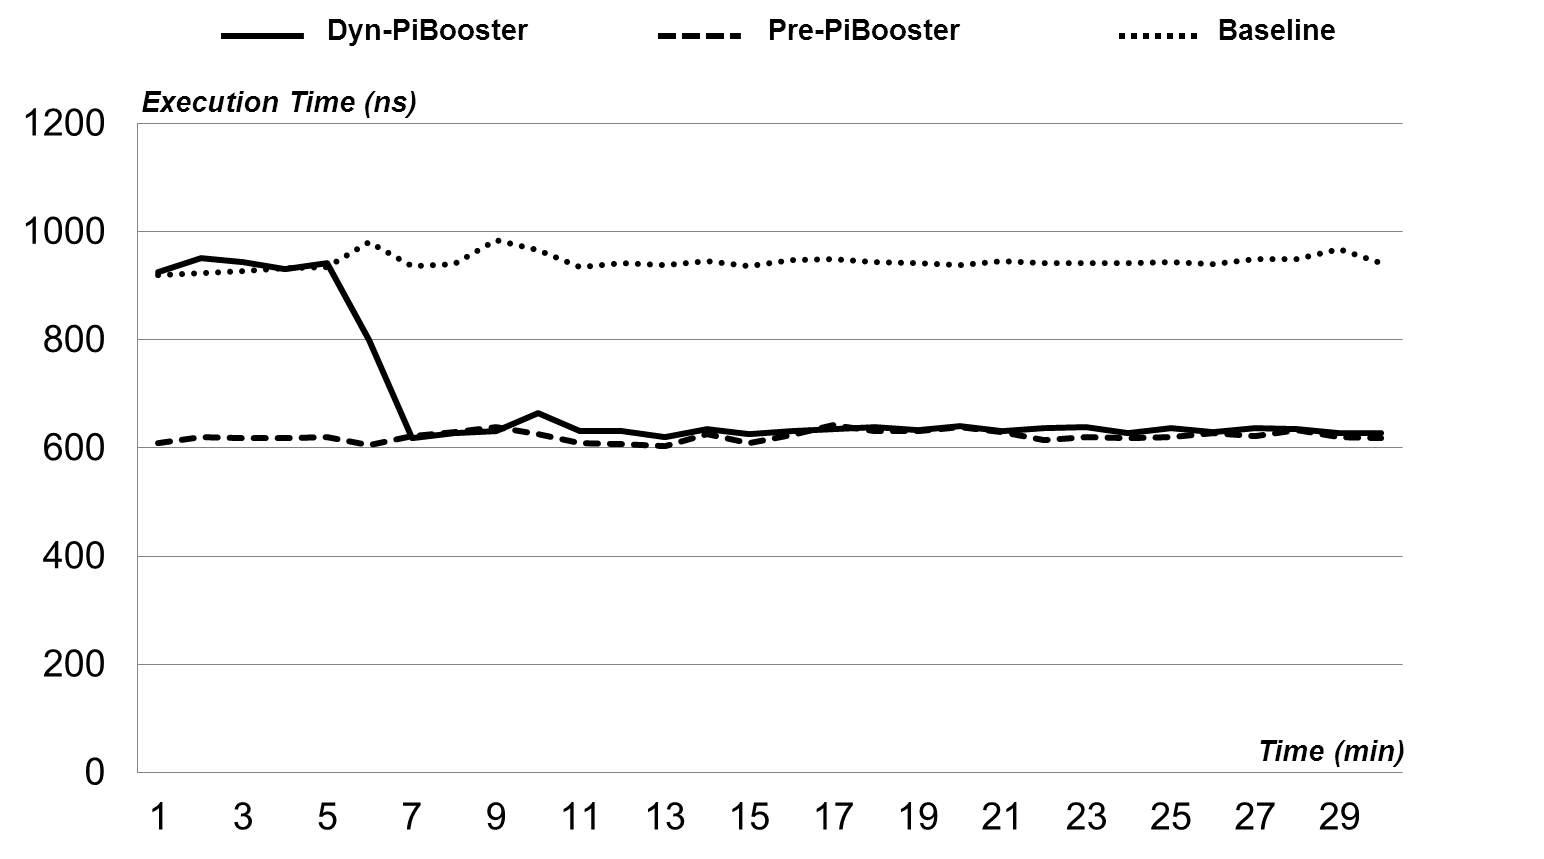
\includegraphics[height=2.0in]{image/micro/PGDalloc.png}
        \caption{Execution time of pgd\_alloc}
        \label{fig:subfig:a}
    \end{subfigure}%
    ~
    \begin{subfigure}[t]{0.5\textwidth}
        \centering
        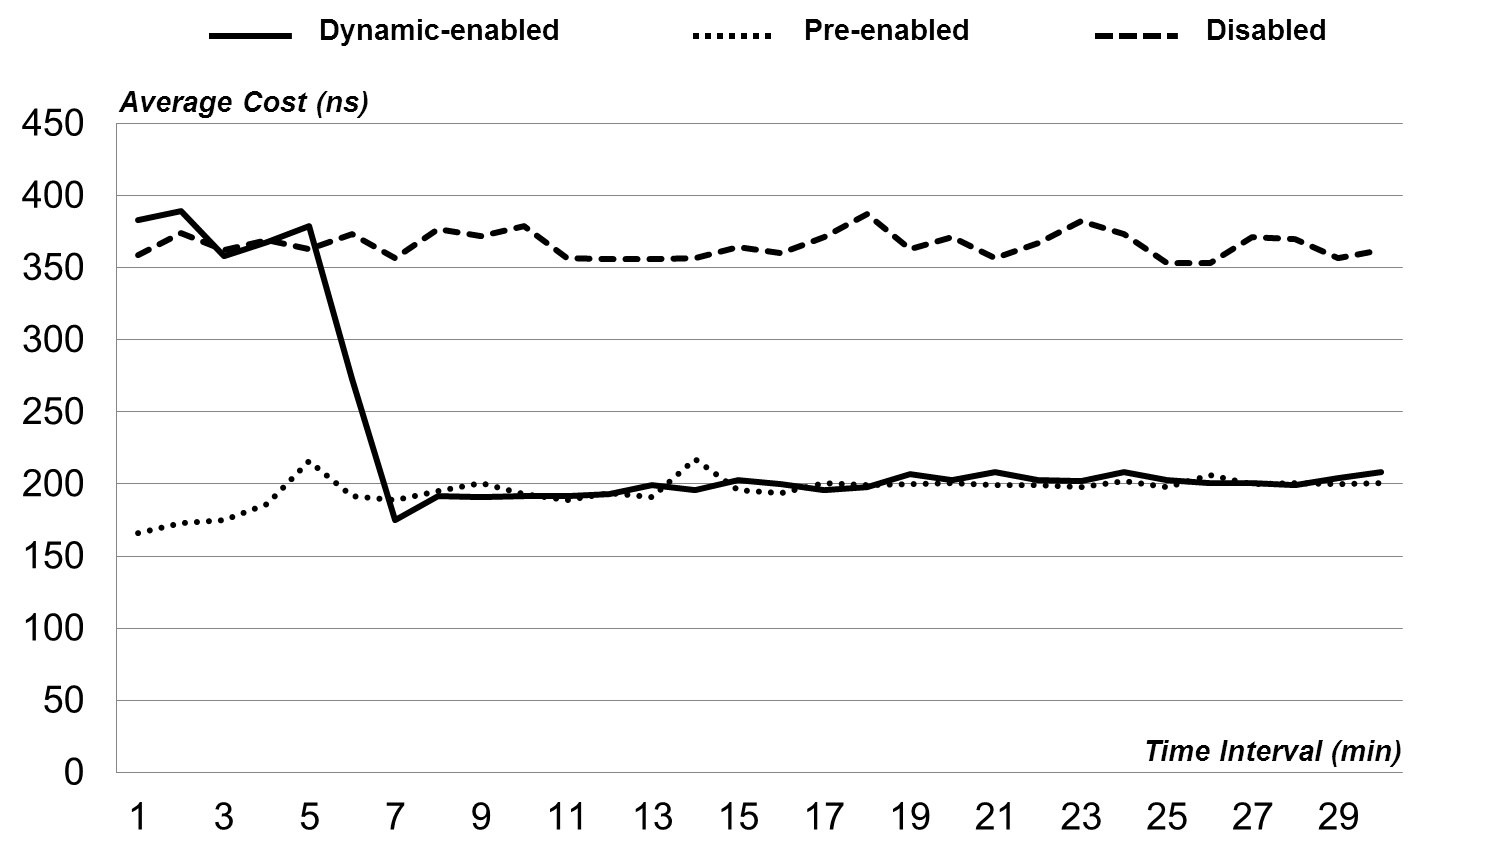
\includegraphics[height=2.0in]{image/micro/PGDfree.png}
        \caption{Execution time of pgd\_free}
        \label{fig:subfig:b}
    \end{subfigure}
    \caption{The time cost in the dyn-\name group is reduced quickly within two minutes to the low level as pre-\name group maintains. And the total execution time of both functions in the pre-\name group is reduced by xx\% compared to that of the baseline group.}
    \label{fig:PGDtime}
\end{figure*}

\begin{figure*}[t!]
    \centering
    \begin{subfigure}[t]{0.5\textwidth}
        \centering
        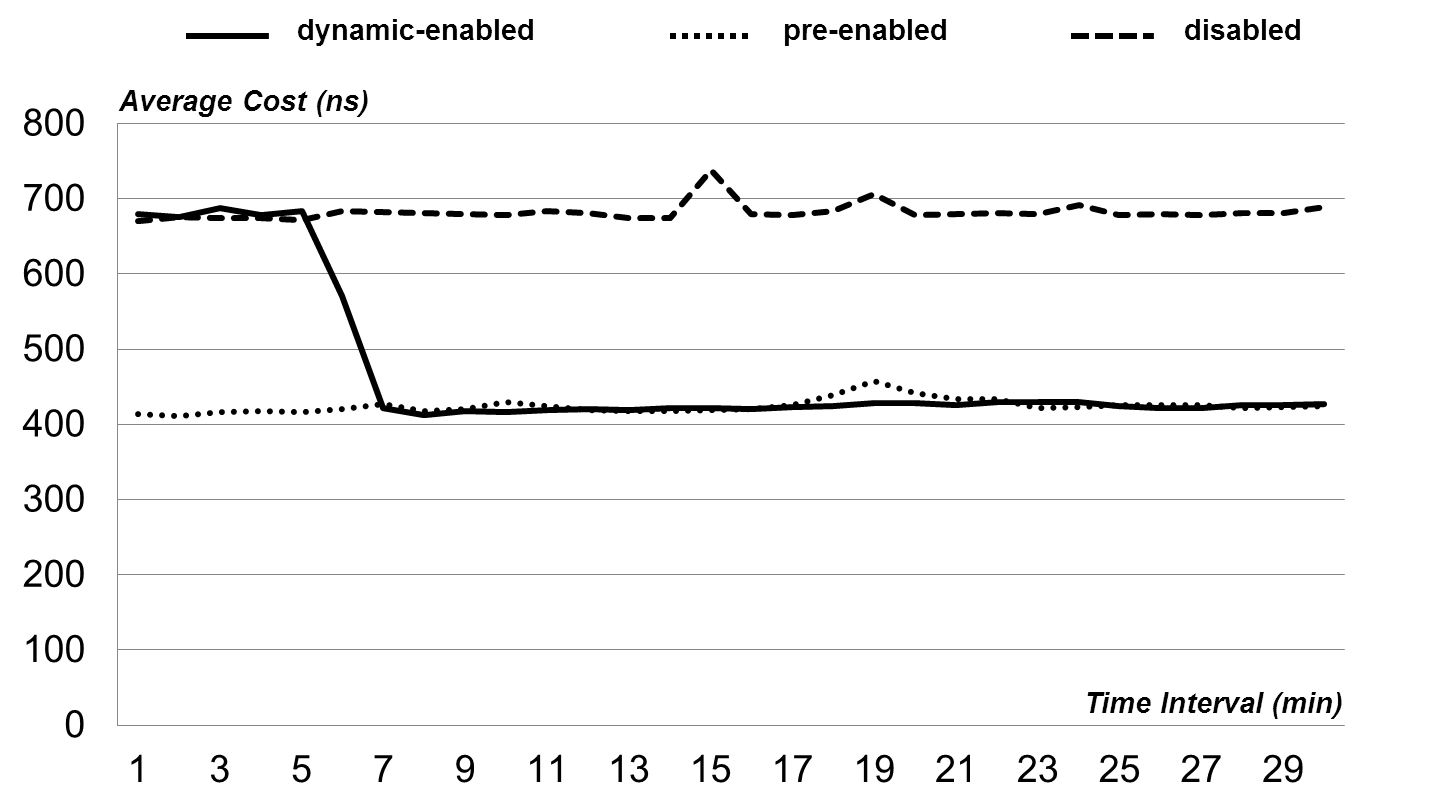
\includegraphics[height=2.0in]{image/micro/PMDalloc.png}
        \caption{Execution time of pmd\_alloc}
        \label{fig:subfig:a}
    \end{subfigure}%
    ~
    \begin{subfigure}[t]{0.5\textwidth}
        \centering
        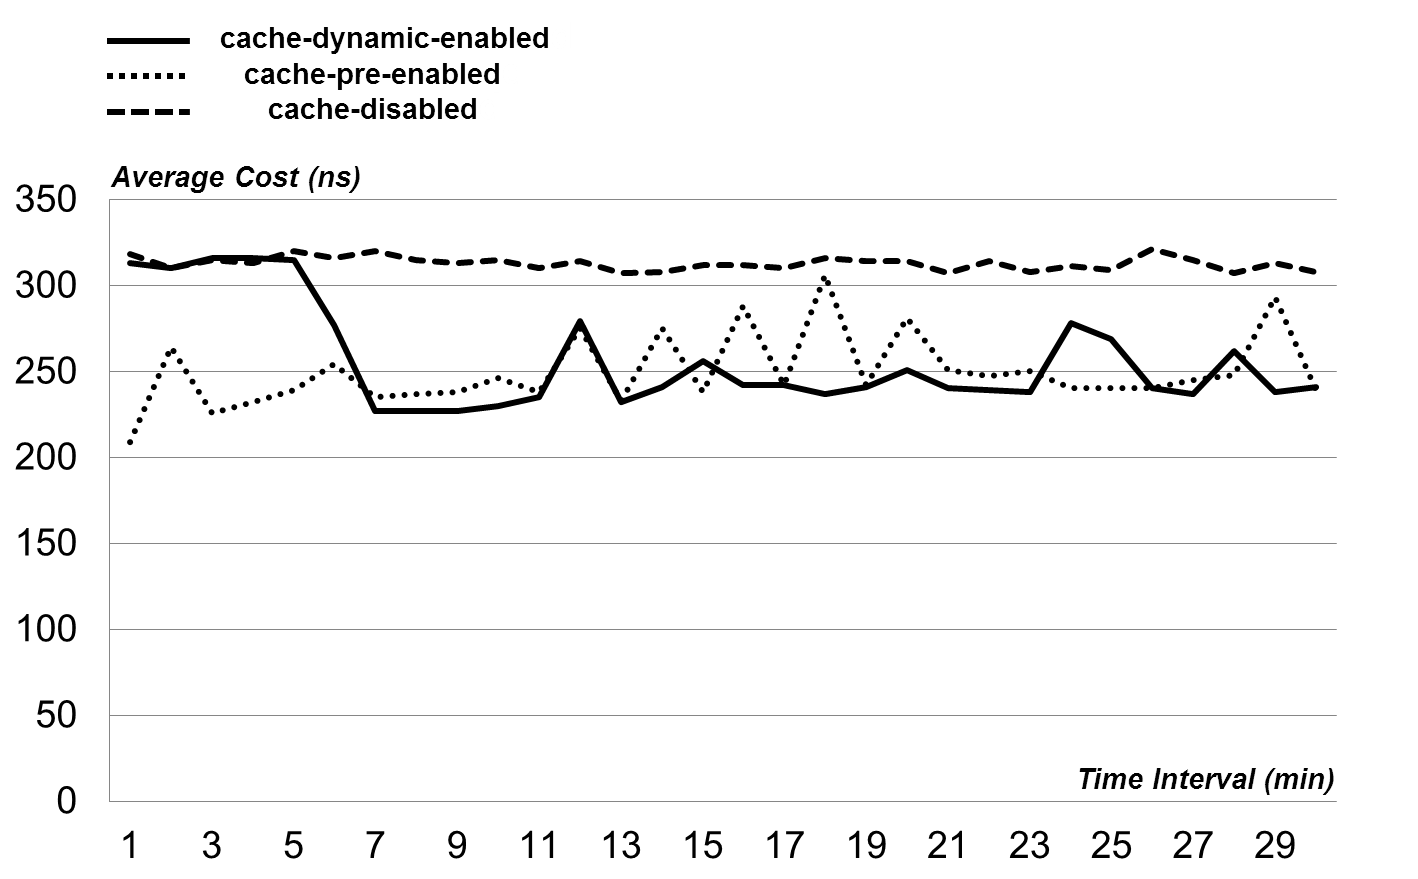
\includegraphics[height=2.0in]{image/micro/PMDfree.png}
        \caption{Execution time of pmd\_free}
        \label{fig:subfig:b}
    \end{subfigure}
    \caption{The trend of time cost in the dyn-\name group behaves like Figure~\cite{fig:PGDtime}. And the total execution time of both functions in the pre-\name group is reduced by xx\% compared to that of the baseline group.}
    \label{fig:PMDtime}
\end{figure*}

\begin{figure*}[t!]
    \centering
    \begin{subfigure}[t]{0.5\textwidth}
        \centering
        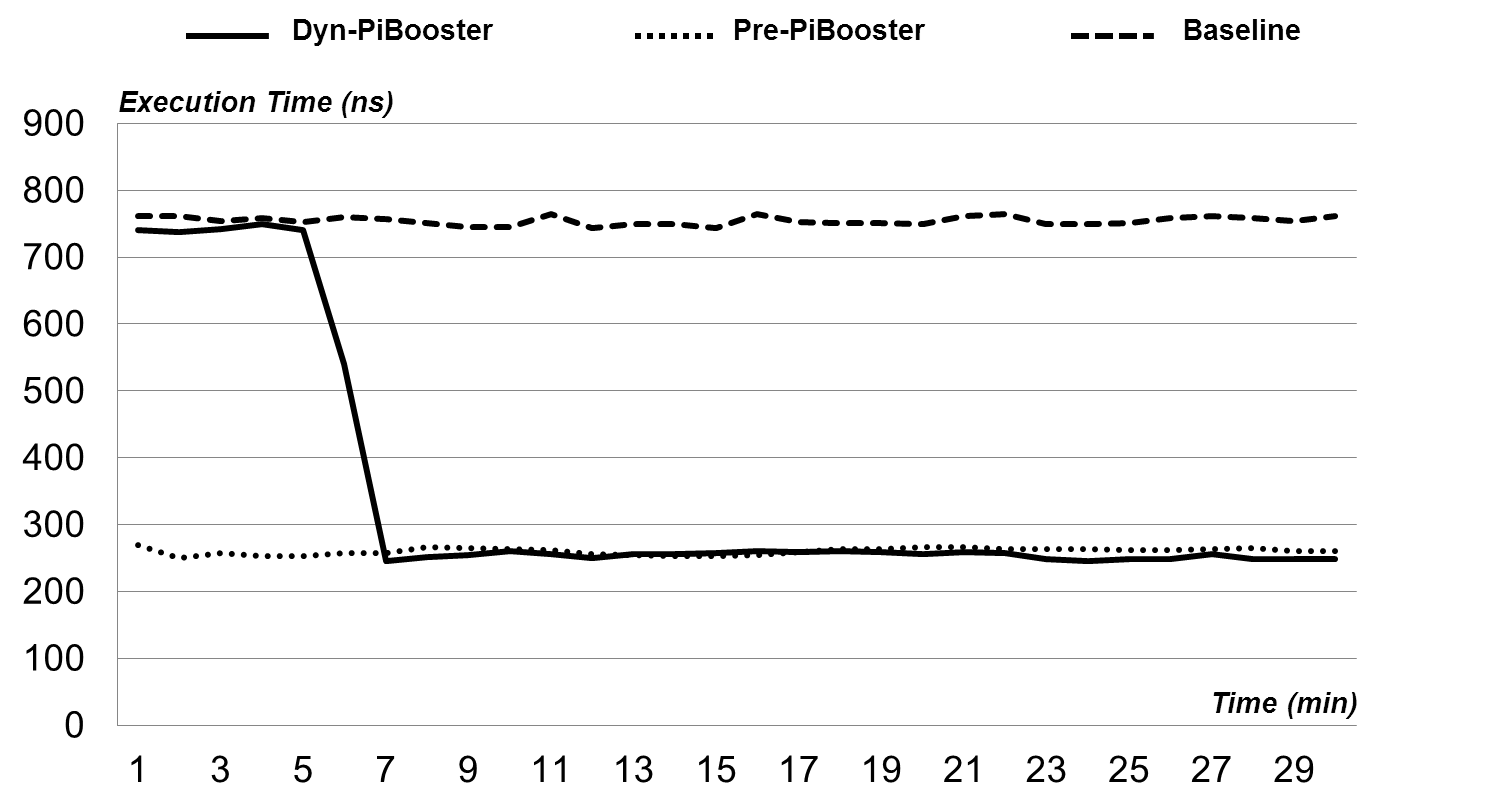
\includegraphics[height=2.0in]{image/micro/PTEalloc.png}
        \caption{Execution time of pte\_alloc}
        \label{fig:subfig:a}
    \end{subfigure}%
    ~
    \begin{subfigure}[t]{0.5\textwidth}
        \centering
        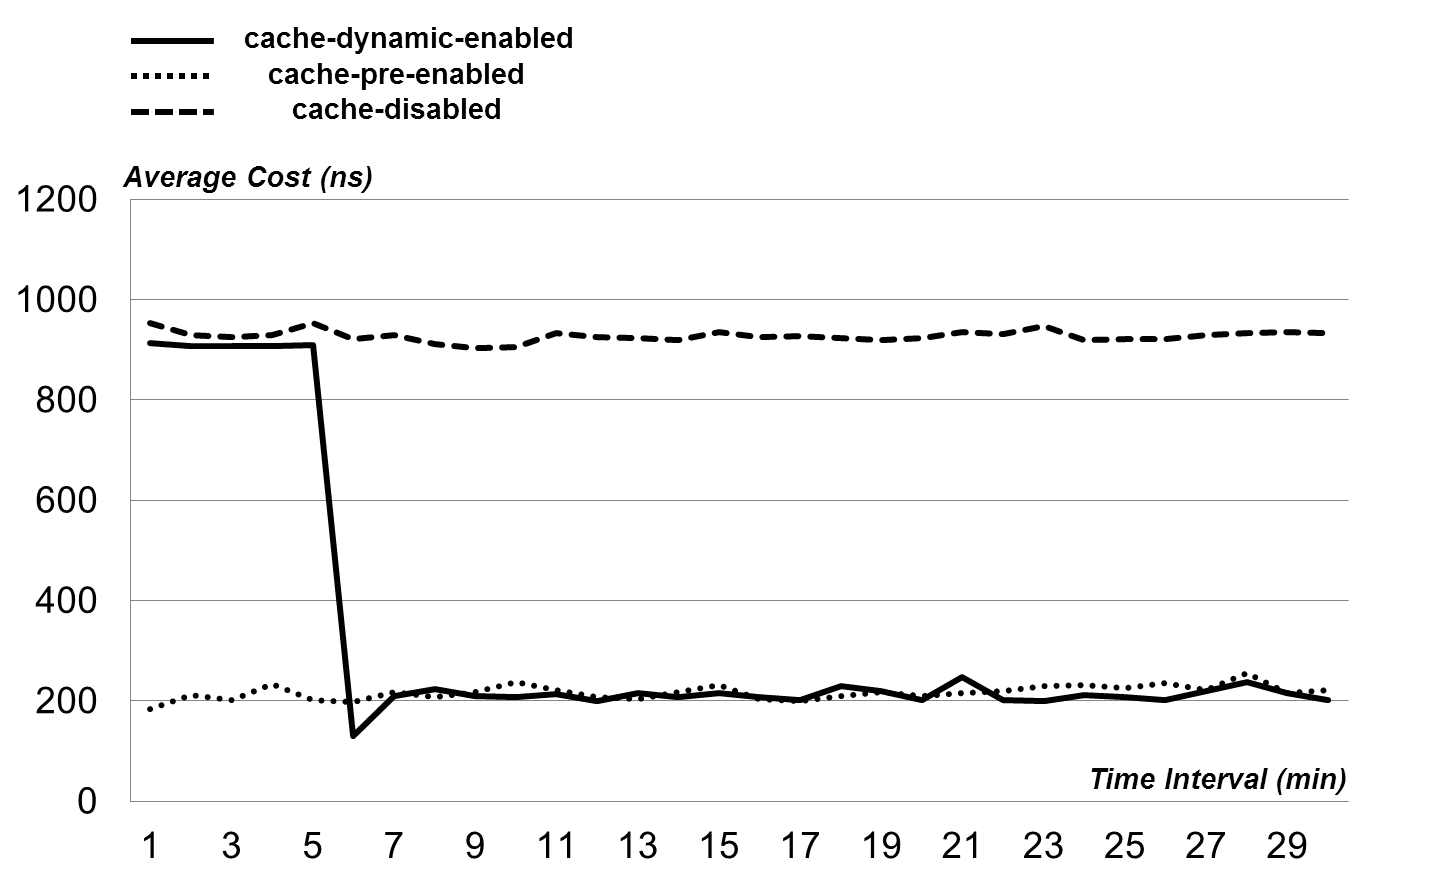
\includegraphics[height=2.0in]{image/micro/PTEfree.png}
        \caption{Execution time of pte\_free}
        \label{fig:subfig:b}
    \end{subfigure}
    \caption{The trend of time cost in the dyn-\name group behaves like Figure~\ref{fig:PGDtime} and \ref{fig:PMDtime}. And the total execution time of both functions in the pre-\name group is reduced by xx\% compared to that of the baseline group.}
    \label{fig:PTEtime}
\end{figure*}

Now let’s move to CPU time that every group will cost. Specifically, each level of page table has its (de)allocation functions, e.g., pgd\_alloc and pgd\_free, and the average execution time of each function is calculated per minute. As shown in Figure~ \ref{fig:PGDtime},\ref{fig:PMDtime},\ref{fig:PTEtime}, both allocation and deallocation functions in all levels of page table in the pre-\name group respectively consume xx\% less and xx\% less CPU time in nanoseconds on average, compared to that of the baseline group, indicating that \name has largely improved the performance of page table (de)allocations by maintaining a dedicated cache.

%When cache is pre-enabled, the ratio between the total pages in cache and the total pages as page tables is approximately equal to 1:1, which indicates that the cache mechanism takes up a small memory percentage of the stress tool.
\begin{table}[!ht]
\footnotesize
\begin{center}
\begin{tabular}{|l|l|l|}
\hline
{\textbf{Page-Table Type}} & {\textbf{Cache (Page \#)}} & {\textbf{Page Table (Page \#)}} \\ \hline
PGD & $5$  & $4$ \\ \hline
PMD & $26$ & $12$ \\ \hline
PTE & $145$ & $177$ \\ \hline
Total & $176$ & $193$ \\ \hline
\end{tabular}
\end{center}
\caption{In the pre-\name group, the ratio between the total cached pages in cache and the page table pages is approximately equal to 1:1 just as expected. And the memory size of cached pages only takes up to xx\% of the tool's memory.}
\label{tab:prePGpool}
\end{table}

\begin{table}[!ht]
\footnotesize
\begin{center}
\begin{tabular}{|l|l|l|}
\hline
{\textbf{Page-Table Type}} & {\textbf{Cache (Page \#)}} & {\textbf{Page Table (Page \#)}} \\ \hline
PGD & $4$  & $2$ \\ \hline
PMD & $20$ & $4$  \\ \hline
PTE & $136$ & $182$ \\ \hline
Total & $160$ & $188$ \\ \hline
\end{tabular}
\end{center}
\caption{In the dyn-\name group, the ratio between the total cached pages in cache and the page table pages is approximately equal to 1:1 as expected. And the memory size of cached pages only takes up to xx\% of the tool's memory.}
\label{tab:dynPGpool}
\end{table}

Besides CPU usage, \name is evaluated in the aspect of memory consumption. Cache size in the pre-\name group shown in Table \ref{tab:prePGpool} reaches only $176$ pages(i.e., ($176 * 4K$) $<$ $1$M) at most in the long time run, only xx\% percentage of the tool's memory (i.e., $284.1$ MB). Besides, memory size in Table \ref{tab:dynPGpool} shows that the dyn-\name group takes up is only $160$ pages at most, also a small percentage of the tool's memory. Both groups consume an insignificant memory usage and reach a satisfying tradeoff between CPU time and memory size. Also note that the conditions of freeing pages in cache in the dyn-\name group heavily rely on a specific scenario, which may not work for other situations. We will further discuss the conditions in future work.

%And the reason why the dyn-\name group has fewer cached pages than that of the pre-\name group is that a certain number of page table pages has been freed to the memory allocator before the \name is enabled.

\mypara{a worst case} As mentioned before, guest kernel firstly goes through \name cache to require enough semi-writable pages when page creations occur. If the cache cannot satisfy the requirements (a.k.a, cache miss), writable pages from the memory allocator will be allocated to corresponding process creations, and these pages will be validated by \name module. Since these pages are judged not to be semi-writable, Xen will enforce both software and DMA protections, which will produce the same number of IOTLB flushes as the baseline. As a result, the execution path of page table allocation in \name in this worst case is longer than that of the baseline. More precisely, \name executes four more instructions than the baseline, and they are two conditional statements, i.e., \name checks if the cache is NULL, \name checks whether the allocated page is semi-writable. Nevertheless, the worse case does not often occur in \name. According to our observations in the dyn-\name group, the probability of cache miss is only xx\% for the thirty minutes since \name is enabled, which indicates that \name performs much better than the baseline in the long-time run.
\zhi{In the pre-\name group, the probabilities of cache miss are 9/550 (0.01\% PGD), 38/2200(0.01\% PMD), 322/6633(0.04\% PTE),respectively. In the dyn-\name group, the probabilities of cache miss are 7/540 (0.01\% PGD), 24/2160(0.01\% PMD), 320/6333(0.05\% PTE),respectively.}


\subsection{Macro-Benchmarks}

Macro-benchmarks are made use of to evaluate the effects of \name on overall system performance. Since dyn-\name group does apply in real cases, macro tests are conducted in two groups, i.e., a baseline group and a dyn-\name group.

\begin{figure}[htp]
\centering
%\includegraphics[scale=0.55]{image/iotlbflush.png} \\
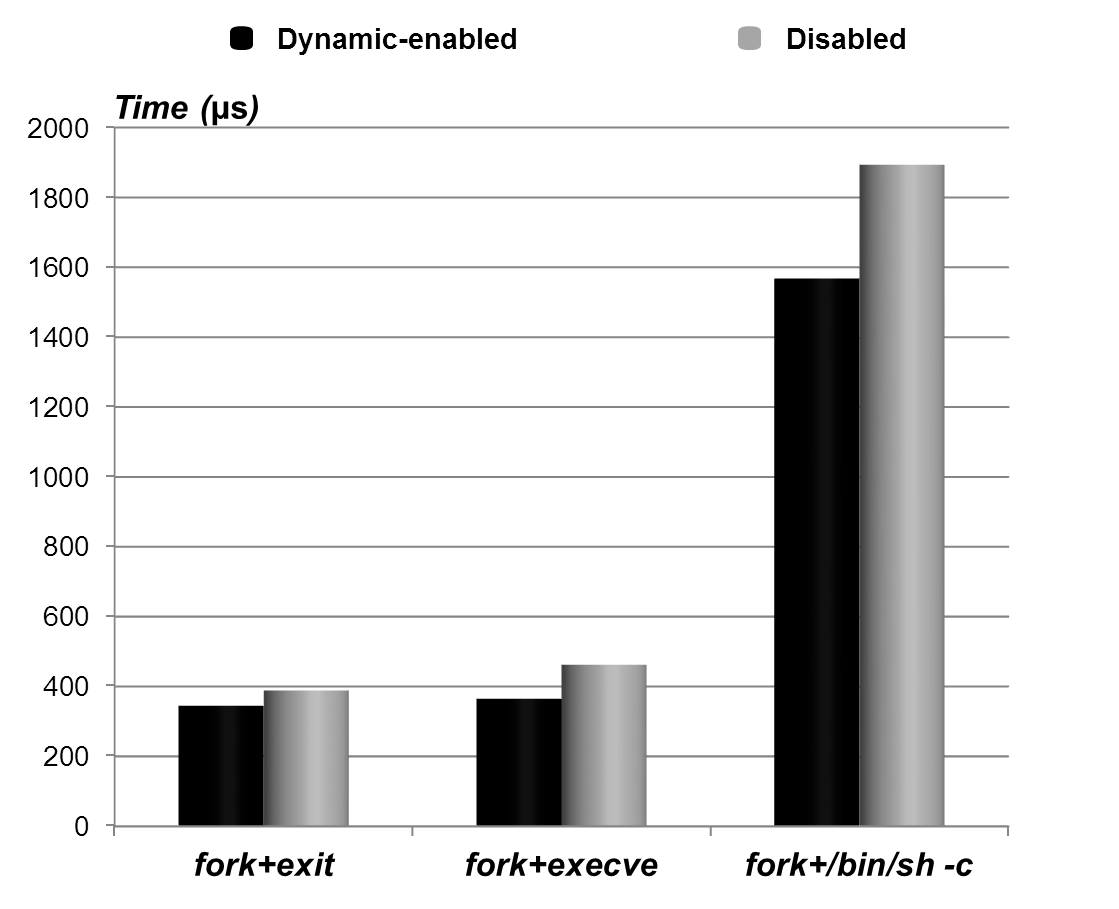
\includegraphics[width=0.5\textwidth]{image/macro/lmbench.png} \\
\caption{The execution time of all processes in the dyn-\name group is reduced by xx\%, compared to that of the baseline group.}
\label{fig:lmbench}
\end{figure}

Lmbench is used to measure CPU time that processes cost (i.e., fork+exit, fork+execve, fork+/bin/sh -c), shown in Figure~\ref{fig:lmbench}. The configuration parameters are selected by default, except parameters of processor MHz, a range of memory and mail result, since CPU mhz of our test machine is $3.2$ GHz rather than the default one, memory range uses $1024$ MB to save time cost of one Lmbench-run and we need no results mailed. As can be seen from the figure, the processes of fork+exit, fork+execve and fork+/bin/sh -c in the dyn-\name group costs $xx$, $xx$, and $xx$ in microseconds, 11\%, xx\%, xx\% fewer than that of the baseline group. Undoubtedly, \name has improved CPU performance.

\begin{figure}[htp]
\centering
%\includegraphics[scale=0.55]{image/iotlbflush.png} \\
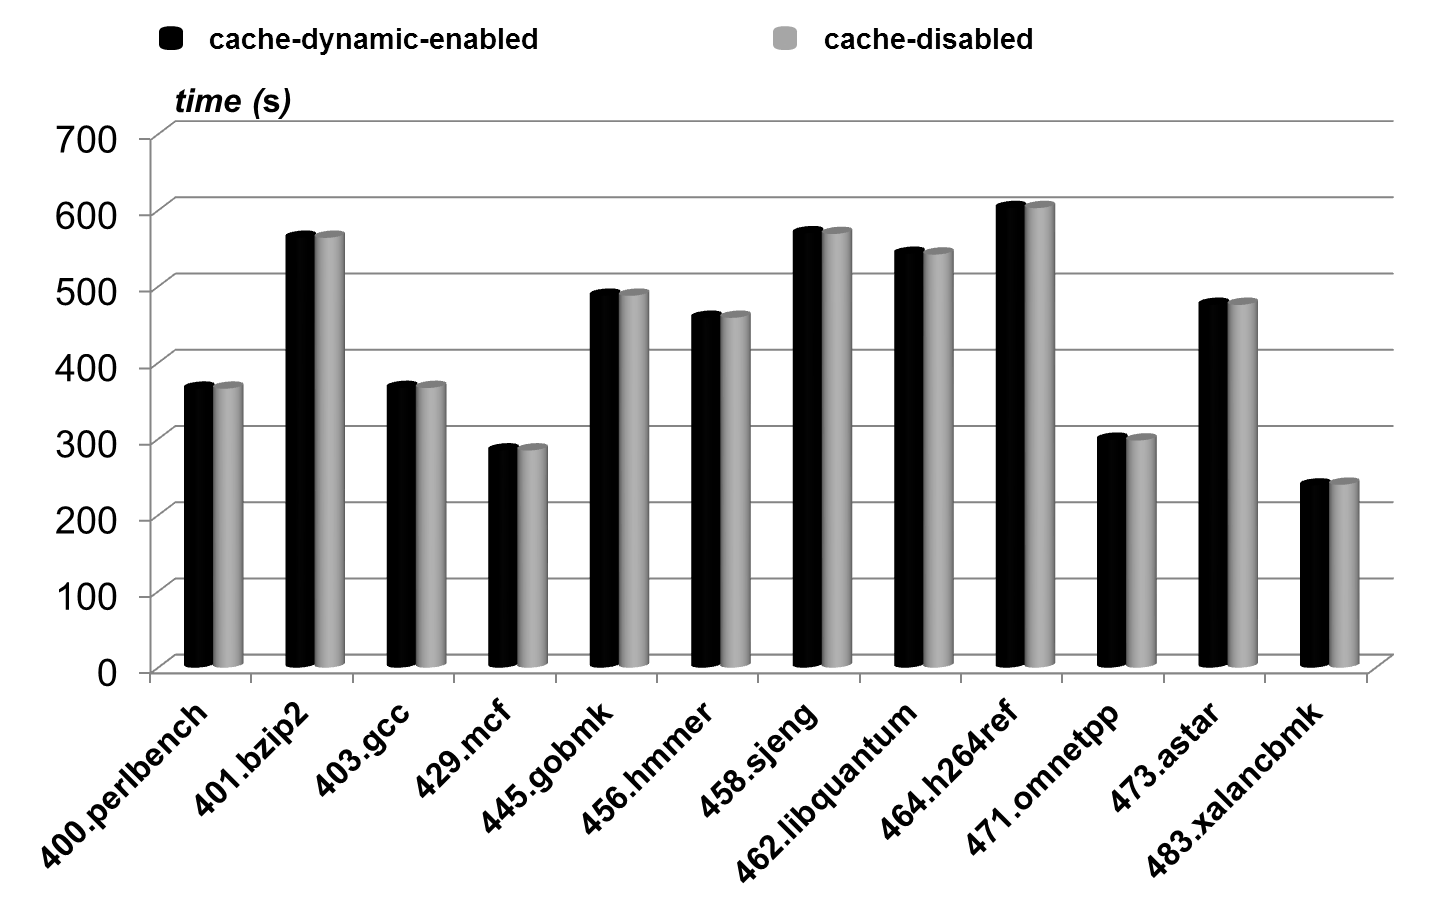
\includegraphics[width=0.5\textwidth]{image/macro/spec.png} \\
\caption{the maximum difference among all the benchmarks is within 0.42\%, indicating that system performance produced by \name is almost the same as the baseline.}
\label{fig:spec}
\end{figure}

SPECint\_2006v1.2 has $12$ benchmarks in total and they are all invoked with EXAMPLE-linux64-ia32-gcc43+.cfg for integer computation, results of which produce Figure~\ref{fig:spec}. Among the benchmarks, the time costs between the two groups vary little and the maximum difference is within 0.42\%, which is produced by the 483.xalancbmk. In the dyn-\name group it costs $239$ seconds, 0.42\% fewer than that of the baseline group, which poses . Thus, the little difference between the two groups indicates that \name does not impose any bad effect on system performance.



%\begin{figure}[htp]
%\centering
%\includegraphics[scale=0.55]{image/iotlbflush.png} \\
%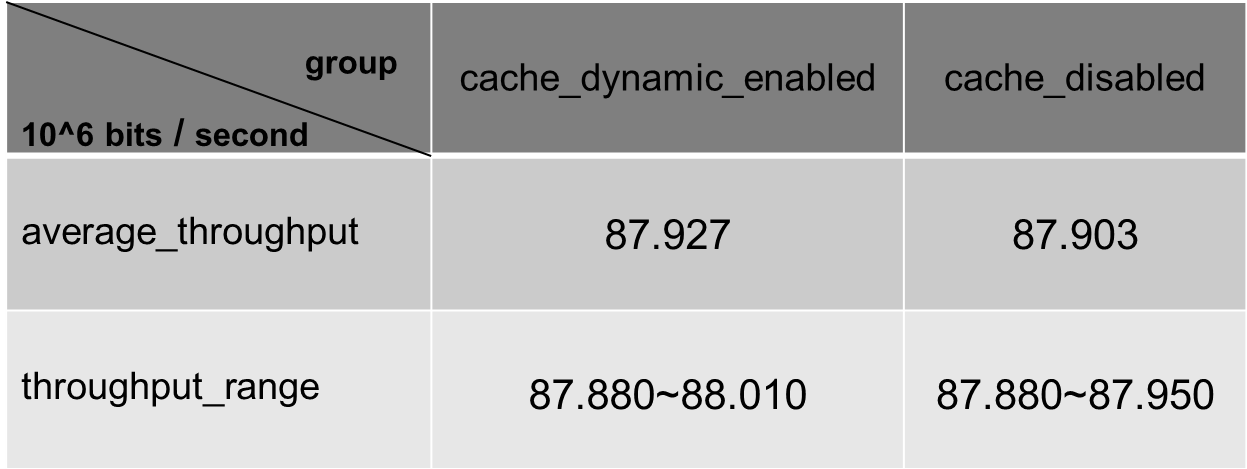
\includegraphics[width=0.5\textwidth]{image/macro/netperf.png} \\
%\caption{Netperf}
%\label{fig:netperf}
%\end{figure}
%|p{1.7cm}|p{1.8cm}|p{1.7cm}


%\begin{figure*}[!t]
%\centering
%\subfigure[PGD Alloc]{
%\label{fig:subfig:a}
%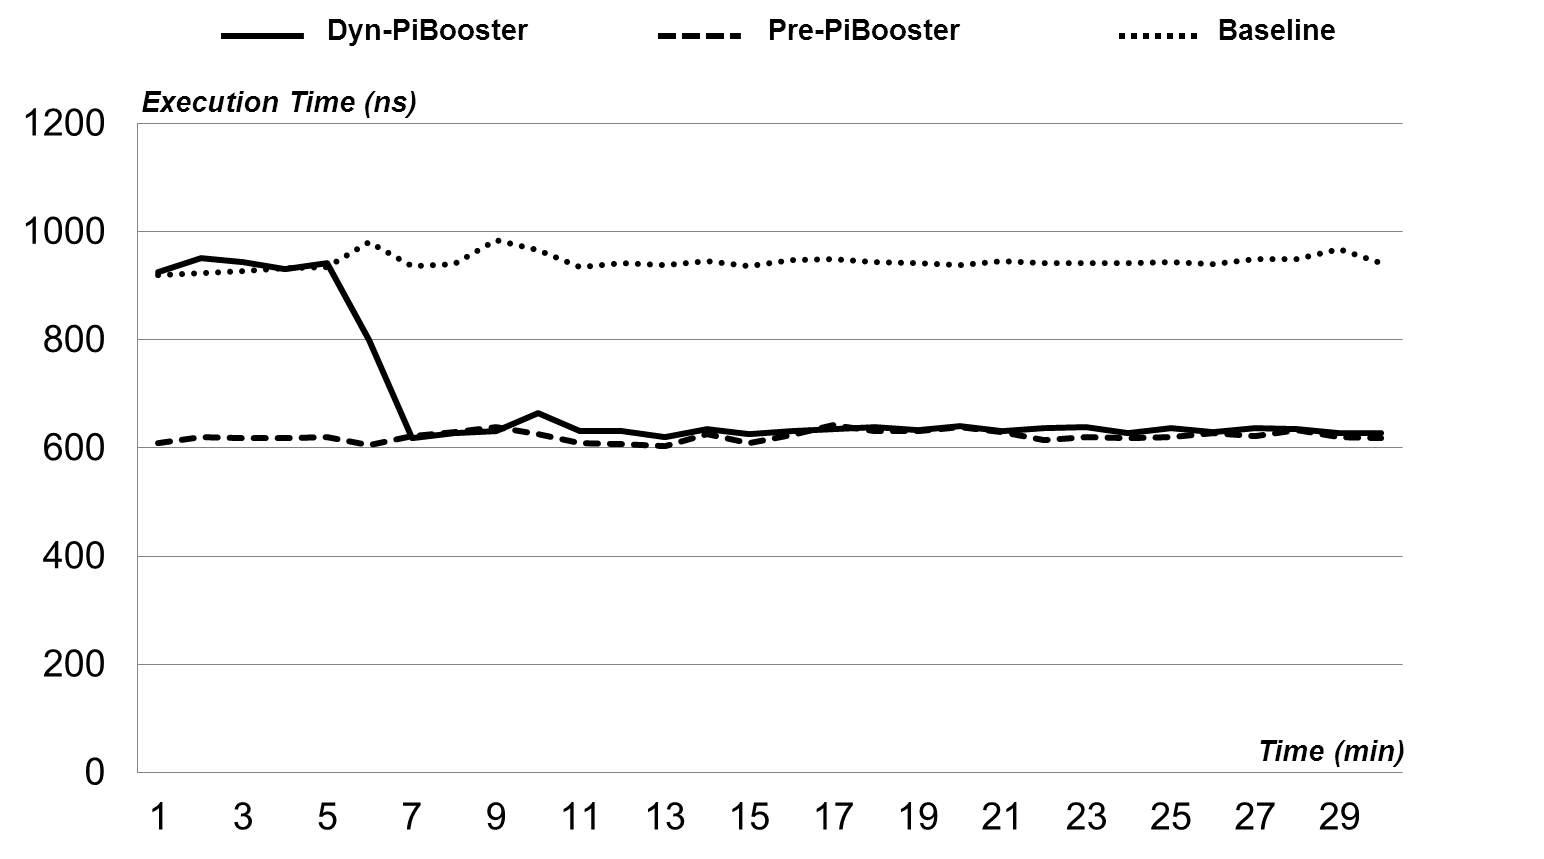
\includegraphics[width=0.5\textwidth]{image/micro/PGDalloc.png}}
%\hspace{1in}
%\subfigure[PGD Free]{
%\label{fig:subfig:b}
%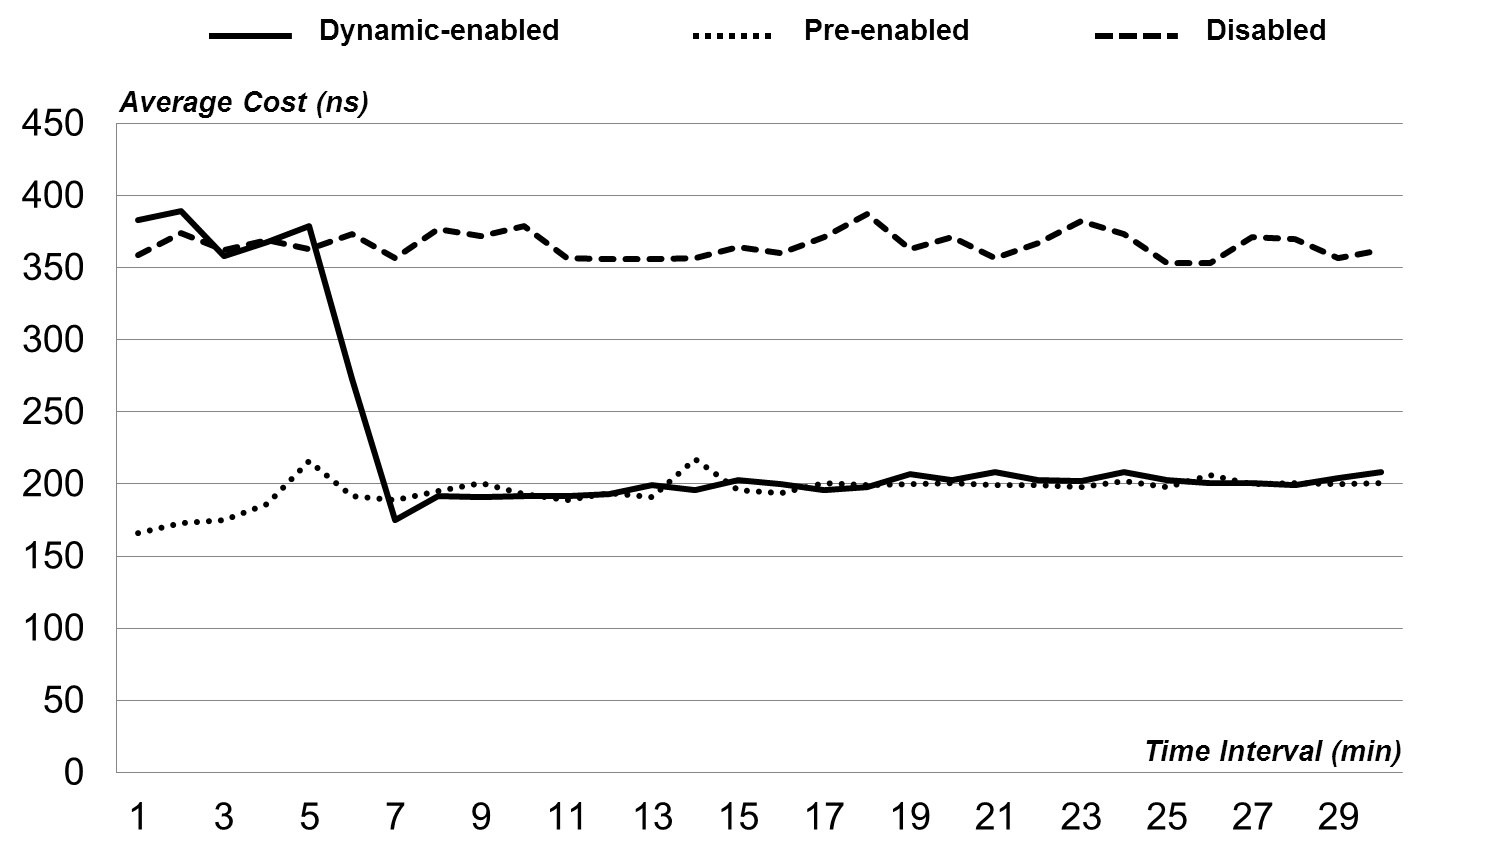
\includegraphics[width=0.5\textwidth]{image/micro/PGDfree.png}}
%\caption{Both page-table cache groups costs much less CPU cycles}
%\label{fig:PGDtime} %% label for entire figure
%\end{figure*}

%\begin{figure}
%\centering
%\subfigure[PGD]{
%\label{fig:subfig:a}
%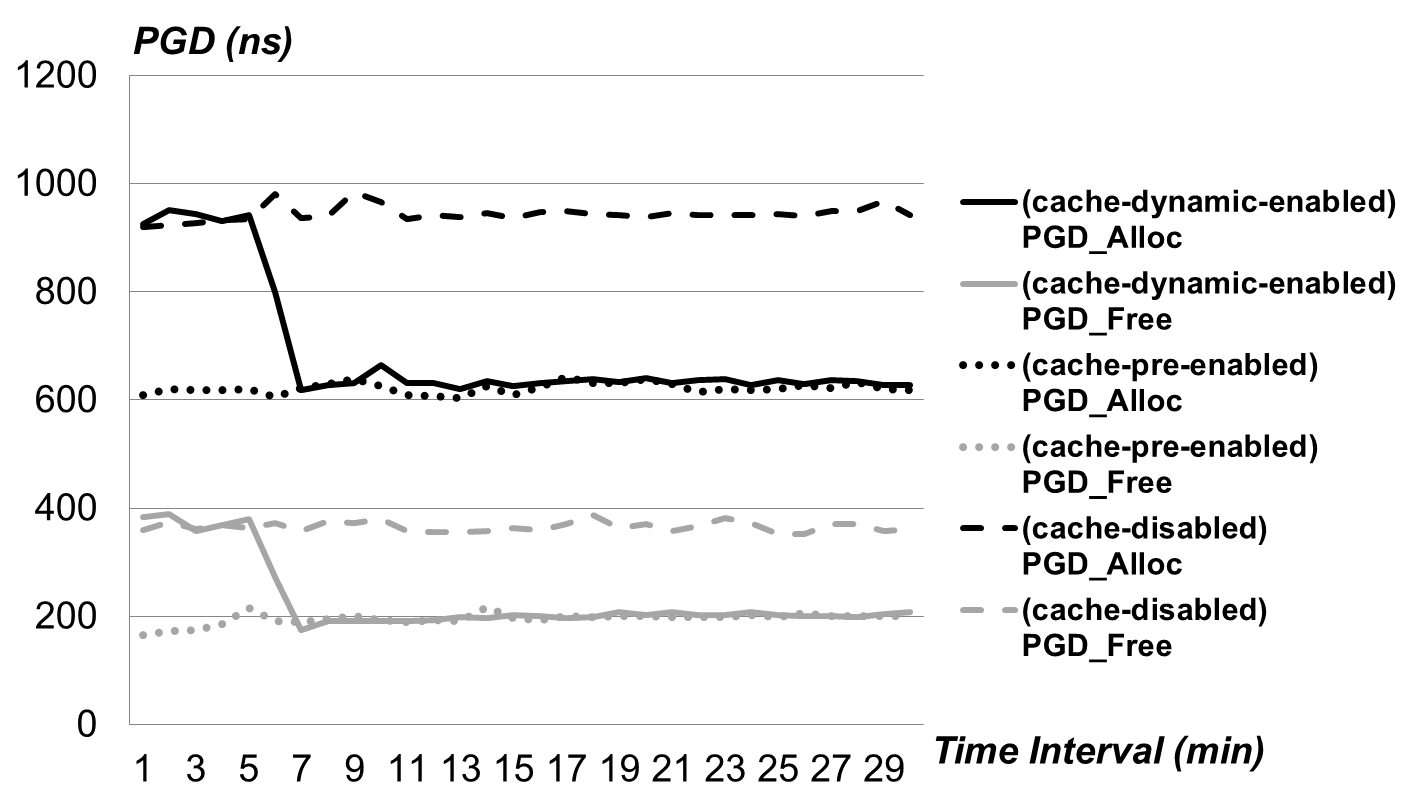
\includegraphics[width=0.5\textwidth]{image/micro/PGDtime.png}}
%\hspace{1in}
%\subfigure[PMD]{
%\label{fig:subfig:b}
%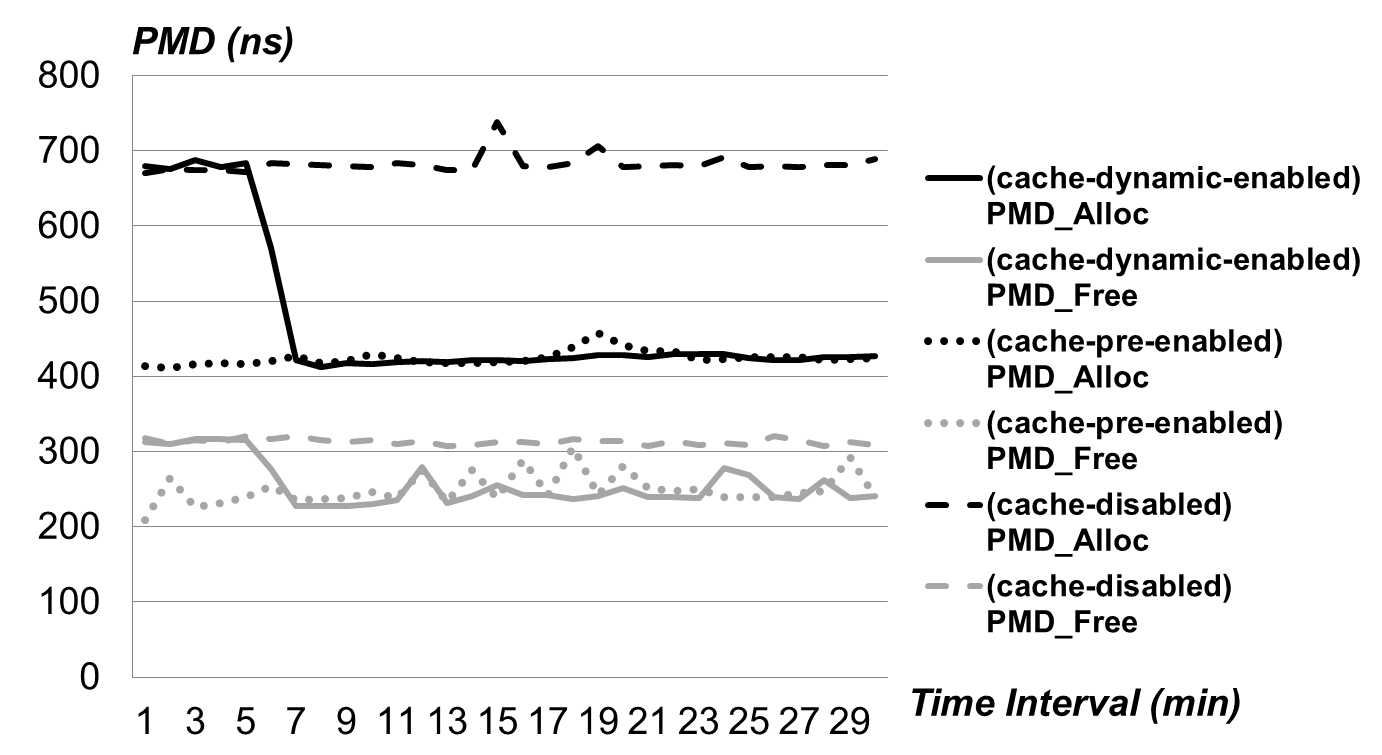
\includegraphics[width=0.5\textwidth]{image/micro/PMDtime.png}}
%\hspace{1in}
%\subfigure[PTE]{
%\label{fig:subfig:c}
%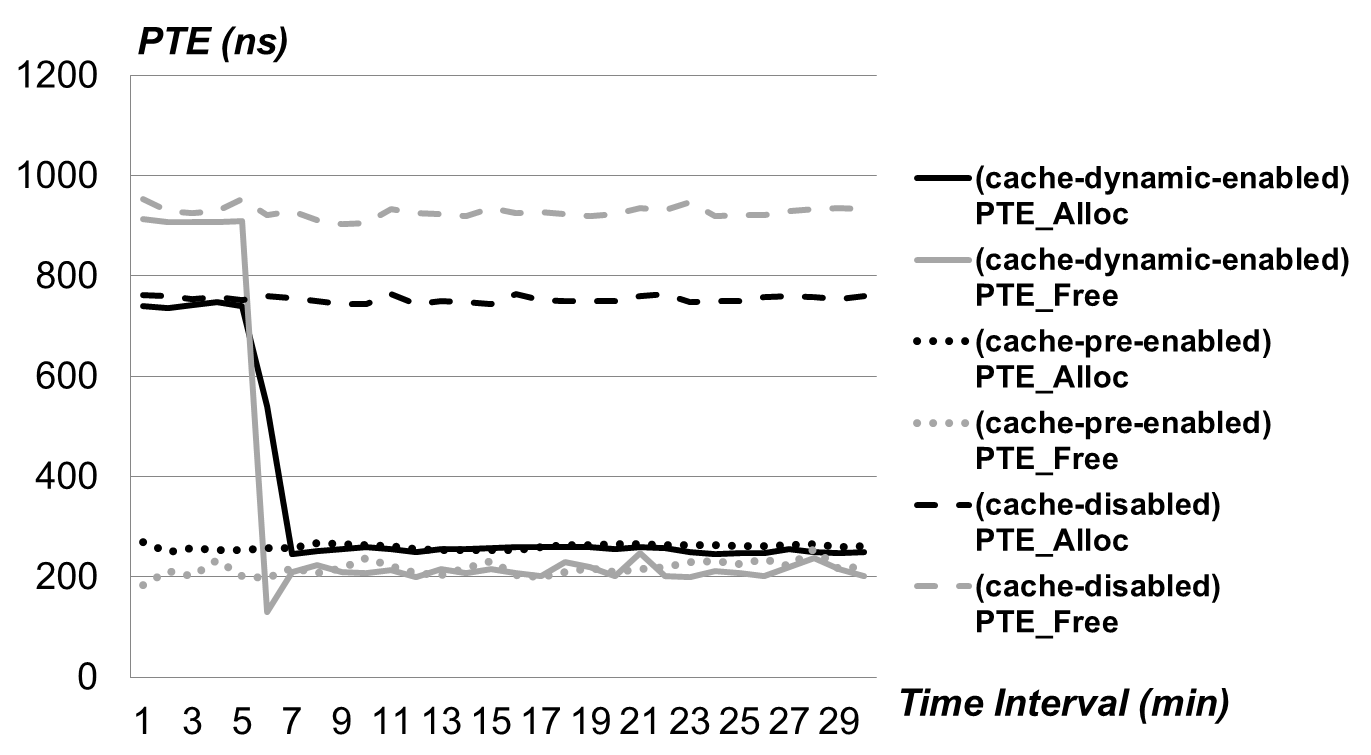
\includegraphics[width=0.5\textwidth]{image/micro/PTEtime.png}}
%\caption{CPU Usage for Each Level of Page Table}
%\label{fig:PGtime} %% label for entire figure
%\end{figure}

%\begin{figure}
%\centering
%\subfigure[PGD]{
%\label{fig:subfig:a}
%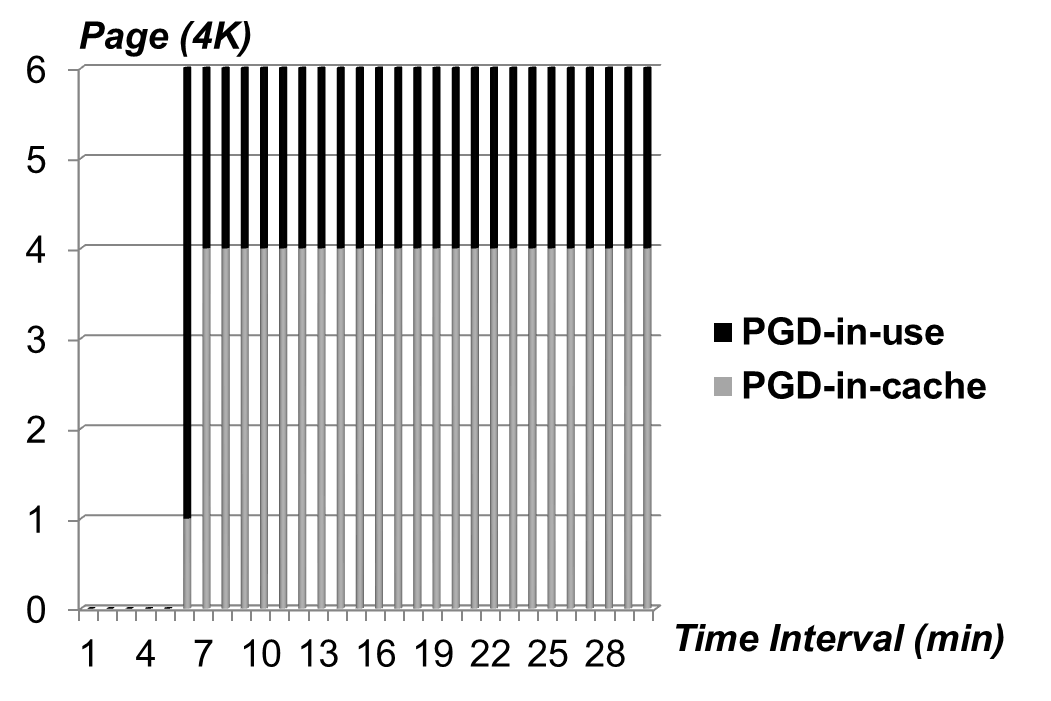
\includegraphics[width=0.5\textwidth]{image/micro/dyn_PGDpool.png}}
%\hspace{1in}
%\subfigure[PMD]{
%\label{fig:subfig:b}
%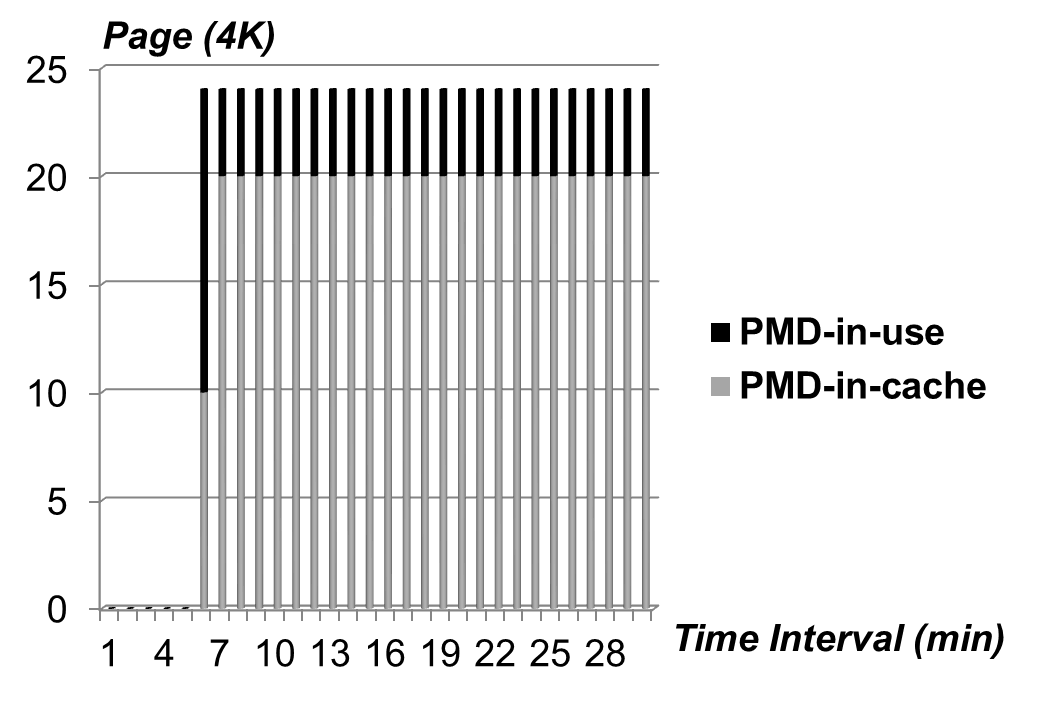
\includegraphics[width=0.5\textwidth]{image/micro/dyn_PMDpool.png}}
%\hspace{1in}
%\subfigure[PTE]{
%\label{fig:subfig:c}
%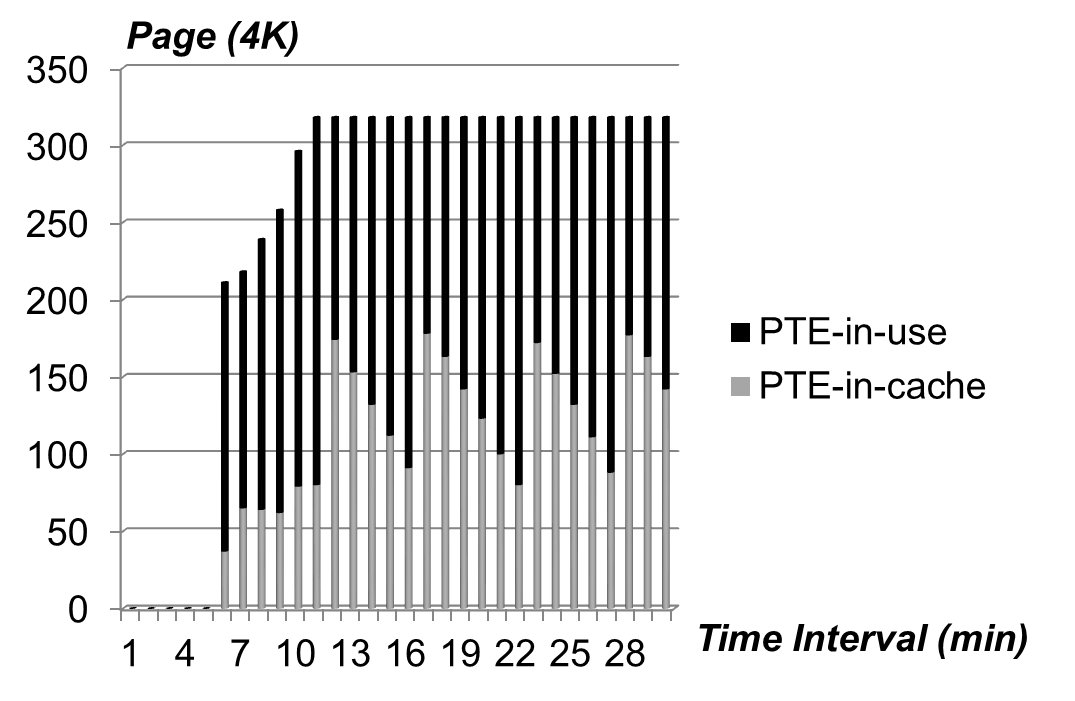
\includegraphics[width=0.5\textwidth]{image/micro/dyn_PTEpool.png}}
%\caption{Cache Pools Size for Cache-Dynamic-Enabled Group}
%\label{fig:dynPGpool} %% label for entire figure
%\end{figure}

%\begin{figure}
%\centering
%\subfigure[PGD]{
%\label{fig:subfig:a}
%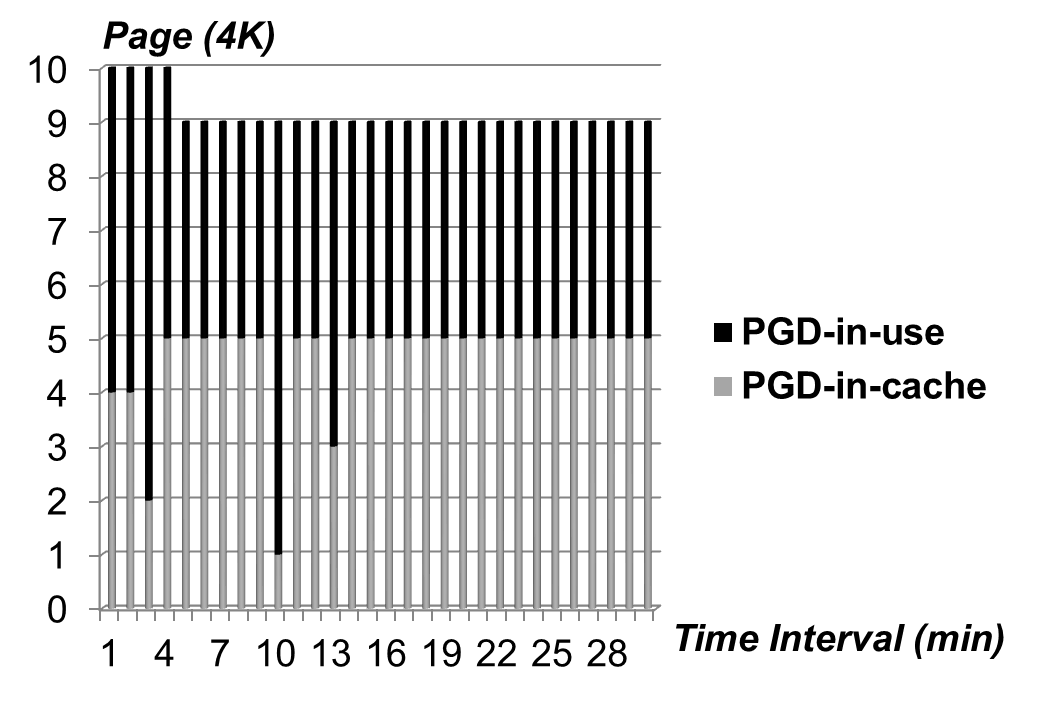
\includegraphics[width=0.5\textwidth]{image/micro/pre_PGDpool.png}}
%\hspace{1in}
%\subfigure[PMD]{
%\label{fig:subfig:b}
%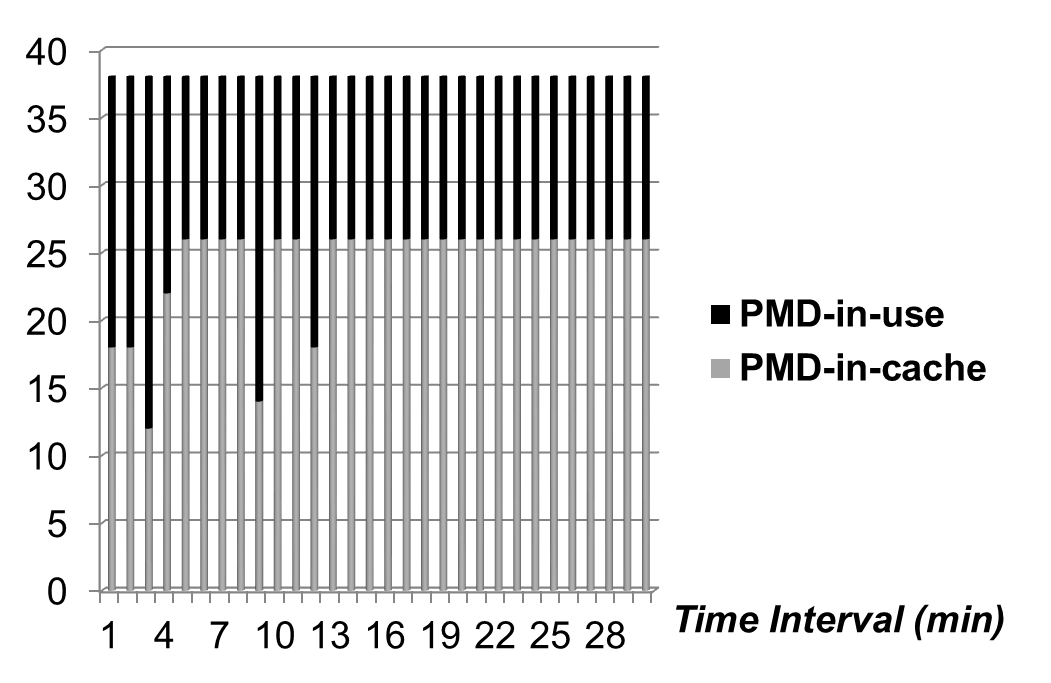
\includegraphics[width=0.5\textwidth]{image/micro/pre_PMDpool.png}}
%\hspace{1in}
%\subfigure[PTE]{
%\label{fig:subfig:c}
%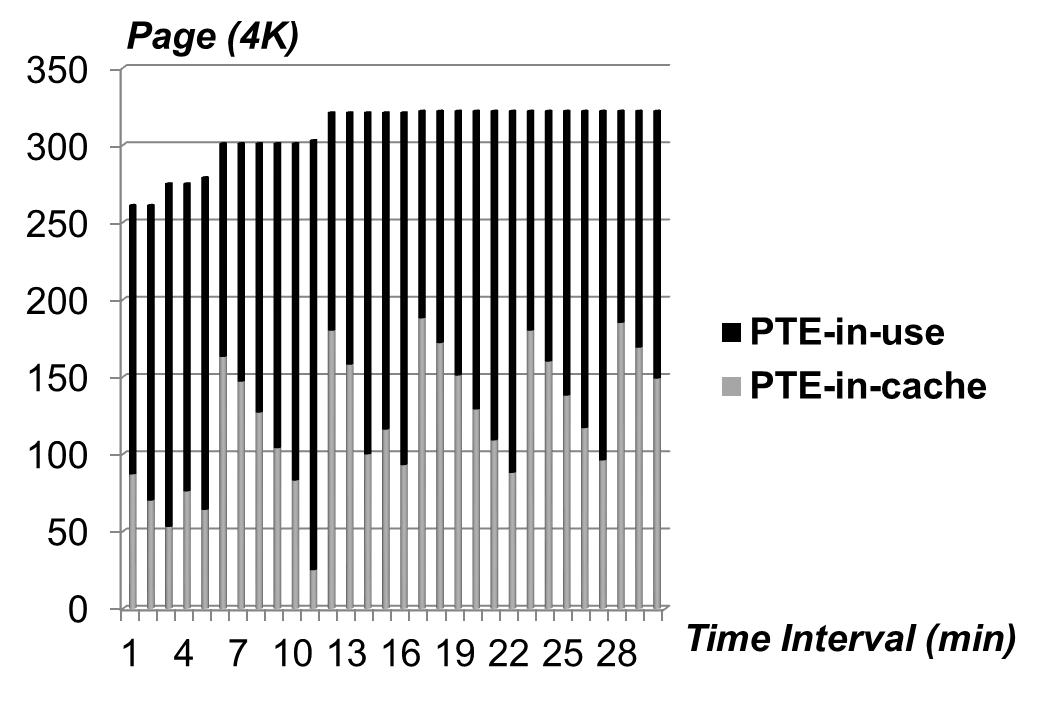
\includegraphics[width=0.5\textwidth]{image/micro/pre_PTEpool.png}}
%\caption{Cache Pools Size for Cache-Pre-Enabled Group}
%\label{fig:prePGpool} %% label for entire figure
%\end{figure}

%PGD & $5$  & $4$   & $>1:1$ \\ \hline
%PMD & $26$ & $12$   & $>2:1$ \\ \hline
%PTE & $145$ & $177$ & $<1:1$ \\ \hline
%Total & $176$ & $193$ & $<1:1$ \\ \hline

%PGD & $4$  & $2$   & $2:1$ \\ \hline
%PMD & $20$ & $4$   & $5:1$ \\ \hline
%PTE & $136$ & $182$ & $<1:1$ \\ \hline
%Total & $160$ & $188$ & $<1:1$ \\ \hline

\section{Discussion} \label{sec:dis}
%\zhi{Macrobenchmark results of netperf do not reveal IOTLB's impacts on the DMA transactions.}
\subsection{IOTLB Impacts on I/O Performance}

Intuitively, IOTLB is used to facilitate the DMA address translation to achieve performance for I/O devices. Therefore, IOTLB misses caused by frequent IOTLB-flush will badly affect I/O performance.

Actually, Nadav Amit \emph{et al.}~\cite{amit2012iommu} claims that IOTLB misses cannot be observed under regular circumstances, since the virtual I/O memory (un)mapping operations consume much more time than that of the corresponding DMA transaction. 

Also, rIOMMU~\cite{malka2015riommu} demonstrates that the overhead caused by walking IOMMU page tables due to IOTLB misses is so negligible that cannot be measured in the netperf benchmark. The benchmark results show that the main latency induced by I/O interrupt processing and the TCP/IP stack is several orders of magnitude larger than that of walking the page tables.

Although it is ascertained that IOTLB has fewer impacts on I/O performance in previous studies, we also use netperf to evaluate IOTLB performance when system is in a \emph{busy state}. To overcome the adverse effect caused by real network jitter, we physically connect the tested machine directly to a tester machine by a network cable, and then the tester machine as a client measures the network throughput by sending a bulk of TCP packets to the tested machine being a server. Specifically, the client connects to the server by building a single TCP connection. Test type is TCP\_STREAM, size of sending buffer is $16KB$ and the connection lasts $60$ seconds. On top of that, the TCP\_STREAM test of netperf is conducted for $30$ runs, results of which are shown in figure\ref{tab:netperf}. By comparing both values of \mu and \sigma, we can safely conclude that the throughputs in both groups change little and IOTLB misses affect little on netperf, which further supports the viewpoint made by rIOMMU. 

%The slight throughput improvement is possibly because that \name spends less CPU cycles executing netperf. Seemingly, benefits of IOTLB-flush eliminations have not been observed so far.

%\times 10^6 bits per second ($1 mbps = 10^6 bits per second$)
\begin{table}[!ht]
\footnotesize
\begin{center}
\begin{tabular}{|l|l|l|}
\hline
{\textbf{Throughput (\emph{Mbps})}} & {\textbf{Dynamic-enabled}} & {\textbf{Disabled}}    \\ \hline
Range & $87.880-88.010$ & $87.880-87.950$ \\ \hline
Arithmetic Mean (\mu)  &  $87.927$ & $87.903$ \\ \hline
Standard Deviation (\sigma) &  $87.927$ & $87.903$ \\ \hline
\end{tabular}
\end{center}
\caption{The throughput values in both groups show few differences by comparing both values of \mu and \sigma, indicating that the IOTLB benefits brought by \name have not been observed so far.}
\label{tab:netperf}
\end{table}

How to make IOTLB become a dominant factor? Nadav Amit \emph{et al.} proposes a pseudo pass-through mode of IOMMU and utilizes a high-speed I/O device (i.e., Intel’s I/O Acceleration Technology~\cite{lauritzenintel}) to do DMA copy operations so as to observe the execution time penalty due to IOTLB misses. While rIOMMU makes use of ibverbs library~\cite{ibverbsevaluation,kerr2011dissecting} to measure the cost of an IOTLB miss in high performance settings where execution time is largely reduced.
we believe that \name can play an important role in I/O environments requiring high performance, which will be evaluated in our future work by utilizing the previous approaches and the I/O high-speed device.
%Both studies aim to create high performance settings that reduce the DMA transactions to the magnitude of $\upmu$s so that IOTLB becomes the dominant factor.

\subsection{Conditions of Freeing Pages in Cache}

As talked before, when to free pages in cache relies on both the memory size of the cache and the proportion between the cache size and page-table size. Default thresholds of the two factors are determined by a particular setting created by a specific stress tool. Therefore, both thresholds may not work in other settings. If the thresholds are not set appropriately, freeing pages will occur often, thus causing IOTLB flush. This is why we provide an interface for users to manually modify the default thresholds. Nevertheless, the optimum tradeoff between cache size and IOTLB-flush is not easy to reach only by the simple interface and we plan to propose a self-adaption algorithm in the future work. Basically, the algorithm has the properties as follows.
\begin{enumerate}
\item (P1) Memory usage of the cache is under control.
\item (P2) Frequency of IOTLB-flush will drop to a lowest level.
\item (P3) The frequency will reach the level as soon as possible.
\end{enumerate}

Firstly, an upper limit to the cache size is set based on the memory usage of a target application. Under the limit, the algorithm manages to eliminate IOTLB-flush with a fewest cache usage. By scanning the the frequency of IOTLB-flush periodically, the algorithm will appropriately adjust the cache size based on both the memory pages in cache and in page tables residing in the target application.


%When users dynamically enable the cache for the application, the algorithm is also invoked to record the memory usage by scanning  and then determine the proportion between them. If IOTLB-flush occurs during the period, increase the cache size. If the cache exceeds a particular percentage of , it is not supposed to be any higher even if IOTLB still flushes.



\section{Related Work} \label{sec:related}
%introduce full virtualization, then move onto PV for performance and finally introduce the security and performance issues.
%VMware~\cite{devine2002virtualization} implements a full virtualization of the underlying computer hardware and allows unmodified guest OSes to execute on a hypervisor, which has degraded the system performance. Denali~\cite{whitaker2002scale} is the first to develop paravirtualization techniques to achieve high performance for modified VMs running network services while Xen~\cite{barham2003xen} is intended to support real operating systems hosting industry standard applications, which makes Xen become popular and widely used in cloud computing. And how to improve its security and performance becomes a major concern.

%talk about how to improve Xen's security.
%Murray \emph{et al.}~\cite{disaggregation} manage to reduce trusted computing base (TCB) of a Xen-based system, which moves the VM-building component from the privileged VM, namely \emph{Domain 0} into a small and trusted compartment.
%Xoar~\cite{colp2011breaking} is proposed to protect Xen hypervisor by breaking the \emph{Domain 0} into several single-purpose components, and each component is configured to expose its dedicated interfaces to VMs and have the least required-privilege access to the hypervisor, also resulting in a reduction of TCB. CloudVisor~\cite{zhang2011cloudvisor} is introduced to prevent leakage of users's data inside a VM by breaking Xen hypervisor into both a resource management module and a nested security monitor and the monitor is responsible for providing protection to the VMs, largely improving Xen's security.

%improve I/O performance for paravirtual I/O method
%As I/O activity is an important performance factor in virtualized environments, the paravirtual I/O method introduced by Xen is efficient to transfer I/O data. Instead of emulating hardware devices, Xen asks the \emph{backend} of a device running in the \emph{driver domain} to communicate with the \emph{frontend} of that device residing in a guest domain by passing the data info through shared-memory, etc. Har'El \emph{et al.}~\cite{har2013efficient} claim to provide a more efficient paravirtual I/O system by combing a fine-grained I/O scheduling and exitless notifications with separate cores, each core dedicated to handling one domain's I/O requests. Besides, to approach bare-metal performance for VMs that interact with I/O devices directly, ELI~\cite{eli} is presented to remove the hypervisor from the I/O interrupt handling path while handle the interrupts within VMs securely.

%talk about IOMMU performance when it is armed by Xen
%As the paravirtual I/O method is not secure enough for DMA access~\cite{disaggregation}, IOMMU (AMD-Vi~\cite{amdvt} or Intel VT-d~\cite{intelvt}) is armed by Xen to prevent buggy device drivers from overwriting system's memory, which subsequently introduces new I/O performance issues. On top of that, Willmann \emph{et al.}~\cite{willmann2008protection} proposes new strategies for Xen to configure IOMMU in order to reduce I/O performance overhead without sacrificing Xen's security. Particularly, Amit \emph{et al.}~\cite{amit2012iommu} and Malka \emph{et al.}~\cite{malka2015riommu} deeply analyze the role of IOMMU's IOTLB in DMA operations and quantifies bottleneck overhead of IOTLB in the high I/O performance environments.

%introduce our work
%In our work, we are focusing on the page table (de)allocations of paravirtual OS. When an OS is ported to Xen, there exists long execution paths of the guest page table (de)allocations and additional IOTLB flushes due to the security validations for page table (de)allocations. Because of the two performance issues, \name is presented to efficiently cut down the execution length and completely eliminate IOTLB flushes, resulting in better performance for both OS and IOMMU.

%Although the hypervisor provides valuable services for memory access from both sides, it is far from enough.
%so as to reduce the performance degradation for the OS inside a VM while prevent illicit access or faults from the OS, achieving a good tradeoff between performance and safety for software access.
%NoHype~\cite{keller2010nohype}
%in its original design, Xen uses an efficient
%Ben-Yehuda~\cite{ben2008xen} talks about the I/O virtualization of Xen by IOMMU~\cite{intelvt,amdvt}, which not only allows direct access to I/O devices by untrusted VMs but prevents buggy device drivers from overwriting system's memory, thereby largely improving the system's availability and reliability for DMA access.

%introduce
%In our work, we focus on the paravirtual page table (de)allocations as well as their impacts on the IOTLB performance. The related work will be introduced from the two aspects as follows.
\mypara{Hypervisor Security by Page Table Configuration} The first category of related work is previous studies in protecting hypervisor by configuring page tables. In paravirtualization where the hypervisor and guest OS are sharing the same virtual space, Xen~\cite{barham2003xen} takes the responsibility of validating every update of guest page tables so as to protect itself from any malicious access. Unfortunately, the protection is not secure enough since the page tables are still \emph{writable}. If a page table entry is modified, the memory protection policy enforced by the page table will be subverted. Because of the security threat, Hypersafe~\cite{wang2010hypersafe} proposes a technique of non-bypassable memory lockdown, which disallows any write attempt to the page tables except benign behaviors conforming to security policy. This key technique further protects the hypervisor's code integrity as well its static data, and it has been applied into Xen.
As a result, they typically focus on how to improve hypervisor security by validating page table updates. \name manages to improve the performance of page table (de)allocations. When an OS is ported to the paravirtual hypervisor, there exists long execution paths of the guest page table (de)allocations, \name is presented to efficiently shorten the execution length.

\mypara{Performance Overhead of IOTLB Misses Reduction} This category is about IOTLB miss reduction. Amit et al.~\cite{amit2012iommu} firstly analyze the role of IOMMU's IOTLB in DMA operations and quantifies the performance overhead of IOTLB misses. Then they present new strategies of both software and hardware enhancements to reduce IOTLB miss rate in order to facilitate DMA address resolution. rIOMMU~\cite{malka2015riommu} re-designs the architecture of IOMMU to achieve high performance in DMA transactions, during which the IOTLB misses are also largely reduced. Willmann et al.~\cite{willmann2008protection} proposes new strategies for Xen to re-configure the addressing mode of IOMMU, resulting in fewer IOTLB misses.
Since we have observed that the security validations by Xen during guest page table (de)allocations will lead to lots of IOTLB flushes, \name focuses on eliminating the additional IOTLB misses by a find-grained validation scheme.

\mypara{Performance Improvement for Paravirtual I/O} The last category is to improve the performance of paravirtual I/O in different ways, where the hypervisor provides a software-based device for its VMs.
%Generally, the virtualization is implemented in two ways, i.e., paravirtual I/O and direct I/O.
%\emph{Paravirtual I/O}
The popular paravirtual I/O technique is introduced by Xen, which is used to transfer I/O data efficiently. Instead of emulating hardware devices, Xen uses the \emph{backend} of a device running in the privileged domain to communicate with the \emph{frontend} of that device residing in a guest domain by passing the data information through shared-memory, etc. To further improve the performance of network devices, ~\cite{menon2006optimizing,4734994,santos2008bridging} manage to optimize Xen's paravirtual I/O model, having achieved a large increase of the network throughput. Ongaro et al.~\cite{ongaro2008scheduling} study the impacts of guest scheduling on guest I/O performance in the context of Xen by concurrently running different combinations of processor-intensive, bandwidth-intensive and latency-sensitive workloads. ~\cite{gordon2012towards,har2013efficient} attempt to reduce VM exits~\cite{adams2006comparison} to provide an efficient paravirtual I/O system. ~\cite{liao2008software,liu2009virtualization,shalev2010isostack,landau2011splitx,xu2013vturbo} designate each core to a specific use. For instance, vTurbo~\cite{xu2013vturbo} facilitates I/O processing for virtual machines by offloading the processing to a designated core with a smaller time-slice than usual. 

%\emph{Direct I/O}


%With the aid of IOMMU, virtual machines can interact with devices directly and securely (a.k.a., direct assignment), which enhances the I/O performance. But it is not enough, ELI~\cite{eli} is introduced to remove the hypervisor from the I/O interrupt handling path while handle the interrupts within VMs securely, thereby approaching bare-metal I/O performance.

\section{Conclusion} \label{sec:con}
The paravirtual guest OS has two important performance issues in page table management : 1) the long execution paths of page table (de)allocations and 2) the additional IOTLB flushes introduced by the DMA validations.
In this paper, we proposed the \name system to address the above problems.
We shortened the execution paths of the page table allocations and deallocations by introducing the \cache, which could quickly response to the page table allocation and deallocation requests.
We introduced a fine-grained validation scheme, which successfully eliminated all additional IOTLB flushes and saved the time for the DMA validations, which further reduced the execution paths.
We implemented a prototype of the \name and fully evaluated its performance in miroc- and macro-benchmarks.
The micro experiment results indicated that \name could \emph{completely eliminate} the additional IOTLB flushes in the workload stable environments, and effectively reduced (de)allocation time of the page table by 47\% on average.
The macro benchmarks showed that the latencies of the process creations and exits were expectedly reduced by 16\% on average.
Moreover, the \emph{SPECINT}, \emph{lmbench} and \emph{netperf} results indicated that \name had \emph{no} negative impacts on CPU computation, network I/O, and disk I/O.


%ACKNOWLEDGMENTS are optional
%\section{Acknowledgments}




%Now we get serious and fill in those references.  Remember you will
%have to run latex twice on the document in order to resolve those
%cite tags you met earlier.  This is where they get resolved.
%We've preserved some real ones in addition to the template-speak.
%After the bibliography you are DONE.

%{\footnotesize \bibliographystyle{acm}
%\bibliography{../common/bibliography}}
{
%\footnotesize
\bibliographystyle{plain}
\bibliography{fastio}
}


\end{document}

IOMMUs have been pervasively deployed on paravirtualized systems for the protection of the hypervisor and the security-critical data structures, e.g., the shared page tables. According to our observations, certain updates of the guest VM's page tables that are supposed to be orthogonal to the device I/O performance, would surprisingly lead to a large number of IOTLB misses. It implies that the I/O performance of all peripheral devices will be affected by the seemingly unrelated guest page table updates. Unfortunately, no existing work uncovers this dependency and adjusts the design of the paravirtualized hypervisor and the guest operating system.







